\documentclass[a4paper,12pt]{report}

% character encoding
\usepackage[T1]{fontenc}
\usepackage[english]{babel}
\frenchspacing
\usepackage[margin=2.5cm,left=3.5cm,includeheadfoot]{geometry} 
\usepackage{setspace}
\onehalfspacing
\usepackage{libertinus} % font: Libertinus Serif

% URLs
\usepackage[dvipsnames]{xcolor}
\usepackage{hyperref}
\hypersetup{
	colorlinks=true, %set true if you want colored links
	linktoc=all,     %set to all if you want both sections and subsections linked
	linkcolor=Black,  %choose some color if you want links to stand out
	citecolor=RoyalBlue
}
 
% Bibliography
\usepackage{csquotes}
\usepackage{biblatex}
\addbibresource{references.bib}
\emergencystretch=1em % Overfull hbox in biblatex

\usepackage{wrapfig}
\usepackage{float}

\usepackage{dirtree}
\usepackage{graphicx}
\usepackage{witharrows}
\usepackage{enumitem}
\usepackage{pdfpages}

\usepackage[chapter]{minted}
\usemintedstyle{manni}
\setminted[python]{fontsize=\small, frame=lines}
\setmintedinline[python]{frame=none}

\graphicspath{ {./images/} }
\begin{document}

\begin{titlepage}

\noindent
\parbox[m]{0.2\textwidth}{
 
\includegraphics[width=0.2\textwidth]{elte_logo.eps}
}
\hfill
\parbox[m]{0.7\textwidth}{
    \begin{center}
        \begin{large}
        \textsc{
            E\"{o}tv\"{o}s Lor\'{a}nd University\\
            \vspace{0.5pc}
            Faculty of Informatics\\
            \vspace{0.5pc}
            Department of Software Technology\\
        }
        \end{large}
    \end{center}
}

\vspace{1pc}
\hrule

\vfill

\begin{center}
{\LARGE Program Synthesis With a Stack-Based Concatenative Language}
\end{center}

\vfill

\noindent
\hspace*{0.05\textwidth}
\parbox{0.45\textwidth}{
    {\it Supervisor:}
    \bigskip
    
    {\Large Dr. Pint\'er Bal\'azs}
    \smallskip
    
    Senior Lecturer
}
\hfill
\parbox{0.45\textwidth}{
    {\it Author:}
    \bigskip
    
    {\Large Su Xiaotian}
    \smallskip
    
    Computer Science BSc
}


\vfill

\begin{center}
{\large {\it Budapest, 2021}}
\end{center}

\end{titlepage}



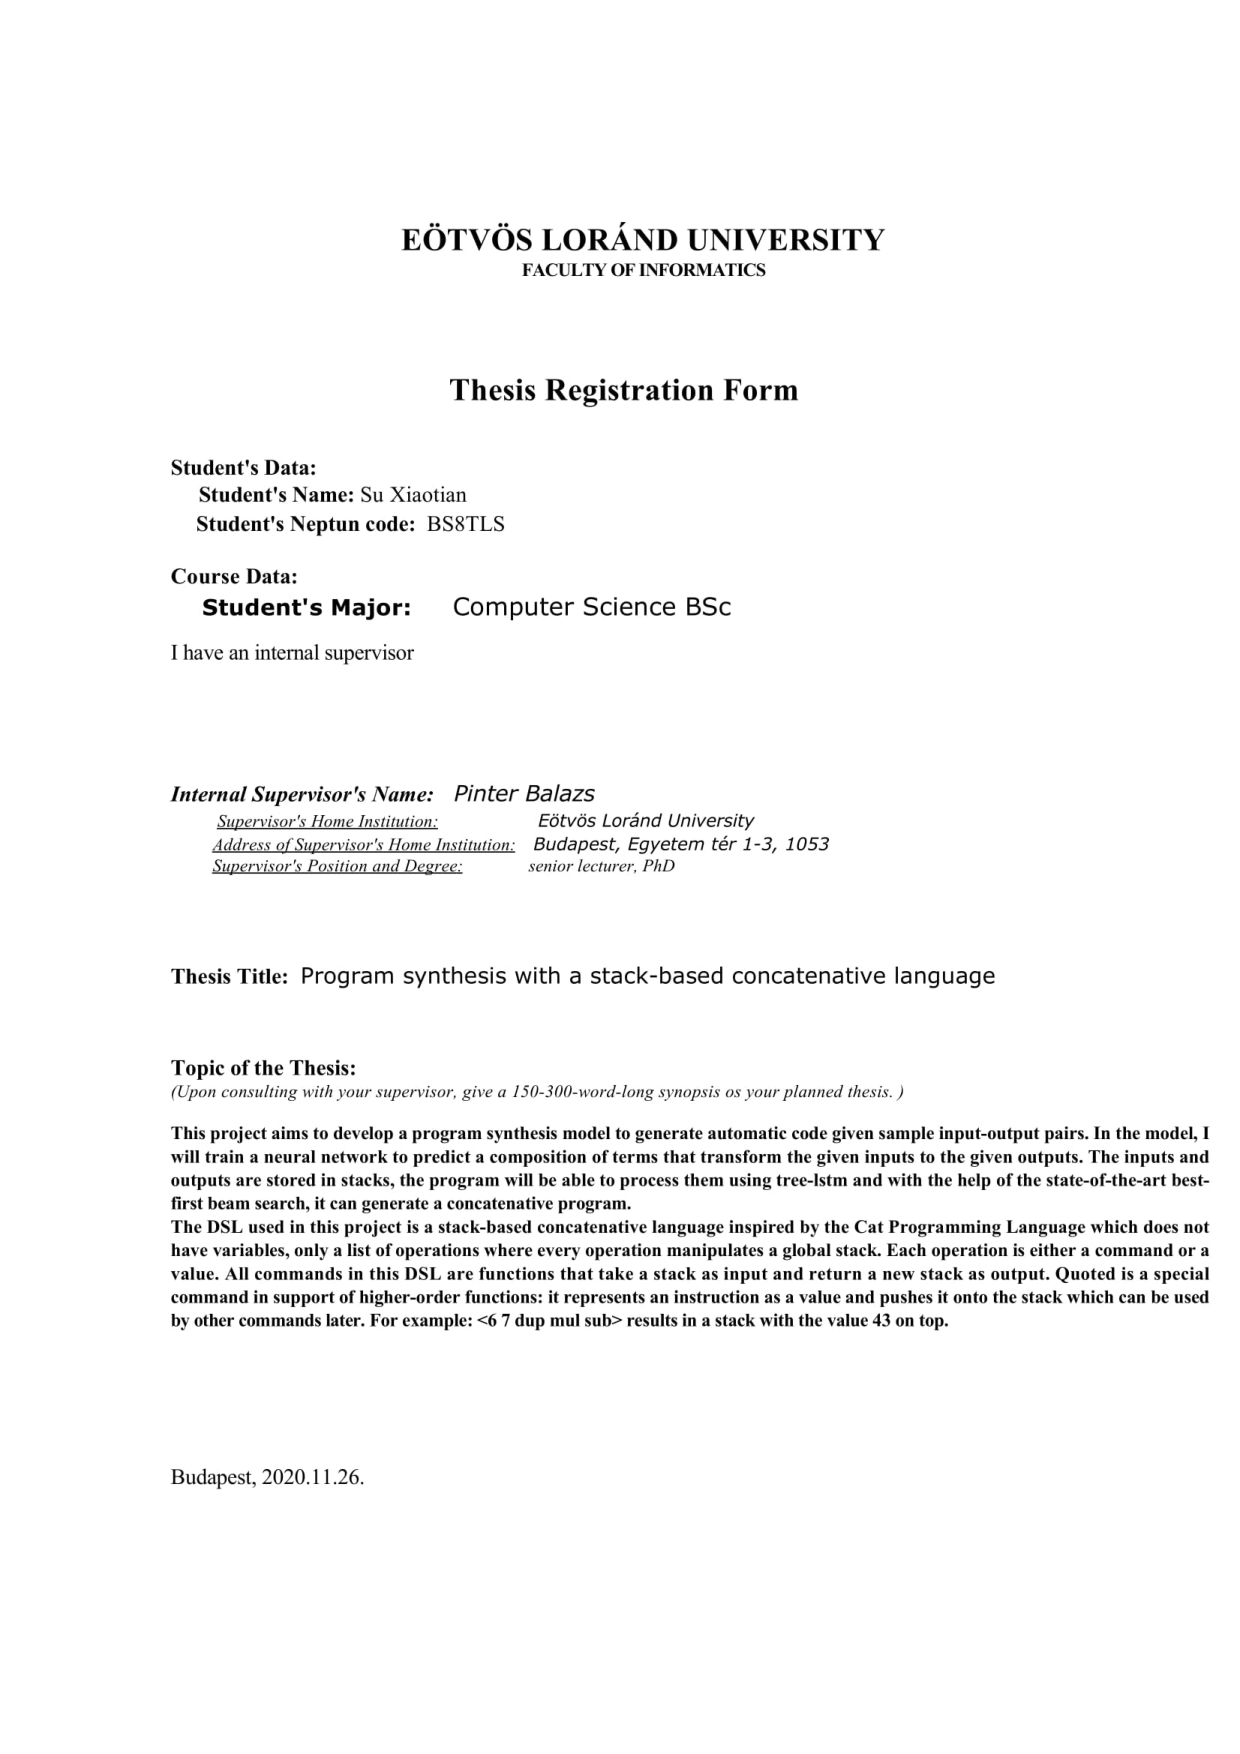
\includepdf[page=1, width=1.3\textwidth]{declaration-1.pdf}

% Table of contents
\tableofcontents

% Chapters
\chapter{Introduction}

Program synthesis is the task of automatically generating code in a particular programming language that satisfies the user intent expressed in the form of some specification. 

This project develops a program synthesis model to automatically construct a program given sample input and output pairs. The program is written in a Domain Specific Language that we constructed on our own.

We first designed and implemented the DSL. Then generating the random stacks and programs. Restrictions to types and values were added during data generation. Afterwards, we embedded the synthetic data into an abstract syntax tree so that they could be fed into the Tree-LSTM network. We trained the model to one term each time that transforms the given inputs to the given outputs. 

The work employs beam search to the program synthesis problem. Given the current state, our neural network directly predicts the next term to manipulate the global stack to get closer to the solution. The beam search algorithm will then rank and select from the network’s outputs, reapplying the predictions at each step. Eventually, we can generate a concatenative program to achieve certain functionalities.

For demonstration purposes, we added a handy graphical user interface with the PySimpleGUI library. The user can enter input and output examples and get the program that satisfies the specification. There is also an animation to exhibit how our DSL manipulates the global stack so as to get the output from the input.

The chapters are as follows: Background (chapter 1) covers the theoretical background practical necessity for program synthesis, the User Documentation(chapter 2) provides detailed guidance for the user to build dependencies and run the program, and the Developer Documentation (chapter 3) covers the necessary knowledge for implementing the domain-specific language, building and training the model, and testing.

\section{Background}
Program synthesis is a field at the intersection of programming languages, formal methods, and AI. It is the mechanized construction of software, dubbed ‘self-writing code’. Synthesis tools relieve the programmer from thinking about how the problem is to be solved; instead, the programmer only provides a description of what is to be achieved. Given a specification of what the program should do, the synthesizer generates an implementation that provably satisfies this specification. Since the inception of artificial intelligence in the 1950s, this problem has been considered the holy grail of Computer Science.\cite{progsynth}

In the thesis, we study program synthesis in a Domain Specific Language (DSL) - a stack-based concatenative language that we implemented on our own, mostly inspired by Cat programming language \cite{cat}. 

Programming languages can be categorized in different ways. One of them is to define the languages as either "concatenative" or "applicative". \cite{concat} In an applicative language, things are evaluated by applying functions to arguments, like C, Python, and Java. In a concatenative programming language, things are evaluated by function compositions. There are no variables in this language, a sequence of operations will take values from an implicit data structure to operate on, and return the result to that structure. This implicit data structure is usually stack. Most existing concatenative languages are stack-based \cite{wiki:concat}. The attributes of the concatenative language make it perfect for chaining existing code to create something new.

A stack-based language is one where most operations are done on a stack of values. Functions take their inputs from the stack, do some computation, and return their results on the same stack. The language often provide some sort of stack manipulation operators. Commonly provided are \texttt{dup}, to duplicate the element atop the stack, \texttt{exch} (or \texttt{swap}), to interchange elements atop the stack. Stack-oriented programming languages may be conceptually difficult for humans to understand, but the advantage is that they are very easy for computers to evaluate and generate. Therefore, it serves as an ideal candidate for the program synthesis project. Section \ref{sec:stack-based} provides a detailed explanation on the stack-based language and Section \ref{sec:stack-based catlang} digs into our DSL. 

\section{Related Work}
The influential work in the field of program synthesis is DeepCoder \cite{deepc} which serves as a baseline for a lot of program synthesis projects. For example, using the Domain Specific Language (DSL) defined by the DeepCoder paper, PCCoder \cite{pcc} showed great advances in the performance of the synthesis process. They managed to solve programs more than two times as complex while preserving decent accuracy and search time. This software used a similar idea as shown in \cite{deepc}, but we constructed our own domain-specific language which is both powerful and neat.

\section{Outline}
Chapter \ref{user} User Documentation has the following content: 
\begin{itemize}
	\item A brief introduction to the main methods and tools used to build the software. See section \ref{sec:tools}.
	
	\item The environment of the developer and how the end-user can install and run the program. See section \ref{install}.
	
	\item The description of the domain-specific language used in the software. See section \ref{sec:lang}.
	
	\item A description of system functions, the running outcome from the user's point of view, and explanation of error messages. \ref{using}
\end{itemize}

\noindent Chapter \ref{dev} Developer Documentation provides the following information: 
\begin{itemize}
	\item An overview of the file structure and workflow of our project. See section \ref{sec:overview}.
	
	\item The importance of domain-specific language and the specification and a detailed explanation of our DSL. See section \ref{sec:dsl}.
	
	\item The process of preparing data before training the model. See section \ref{sec:datagen}.
	
	\item The architecture of our neural network and the selection of hyperparameters and the loss function. See section \ref{sec:network}.
	
	\item Testing plans, tools, writing examples, and results. Pytest \cite{pytest} is for unit testing and hypothesis test \cite{hytest} is used for property testing. See section \ref{sec:test}.
\end{itemize}
\chapter{User Documentation}
\label{user}
This software intends to demonstrate the user how our domain specific language works to manipulate the global stack. In this chapter, the application will be explained from an end-user perspective with demonstration on how to build and run the program and how to enter input-output pairs to get the program that achieve a certain function.

\section{Main Methods and Tools}
\label{sec:tools}
The user interface is written using PySimpleGUI \cite{psgui}, a Python package that enables Python programmers of all levels to create GUIs. PySimpleGUI is currently capable of running on 4 Python GUI Frameworks, they are PySimpleGUI, PySimpleGUIQt, PySimpleGUIWx, and PySimpleGUIWeb. Here we used the default PySimpleGUI Framework. The algorithm that implements the DSL and builds the model is written in Python 3. We used the typing module which was introduced in Python 3.5 \cite{typing} to do the type check and the package PyTorch \cite{pytorch} to build the neural nets.

\section{Installing}
\label{install}
The installation of the software is relatively straightforward and simple. This section will walk the end-user through the process of setting up the environment, installing dependencies, and running the program.

\subsection{Environment}
The development environment is typically a workstation for developers, while the production environment is a real-time setting where programs are run and used by end users. In this project, we will implement the app and run the tests in the development environment.

The specification of the system used to develop this application consists of:
\begin{itemize}
    \item Operating System: macOS Big Sur
    \item Ram: 16.0 GB
    \item CPU: 2.0 GHz
    \item Code Editor: Visual Studio Code
    \item Python 3.8.0 ( requirement: Python 3.5, 3.6, 3.7, 3.8)
\end{itemize}
\subsection{Installation}
We have all the prerequisites written in requirements.txt and environment.yml, you can built dependencies easily with those files in either of the following methods.
\noindent Method 1: If you have \texttt{Python}, \texttt{pip} installed, you can use the following steps:
\begin{enumerate}
	\item 	Open a terminal and change to the project directory.
	\begin{itemize}
		\item Install virtualenv: \texttt{pip install virtualenv}
		\item Create a virtual environment: \texttt{virtualenv venv} 
		\item Activate it: \texttt{source venv/bin/activate}
	\end{itemize}
	
	\item Install the requirements: 
	\texttt{pip install -r requirements.txt}
	
	\item Run the app:
	\texttt{python main.py}
	
\end{enumerate}

\noindent Method 2: If you have \texttt{conda} installed, you can follow the steps below to install the dependencies before running the program:
\begin{enumerate}
	\item Open a terminal and change to the project directory.
	\begin{itemize}
	    \item 	Create an environment: 
	    \texttt{conda env create -f environment.yml}
    	\item Activate the environment:
    	\texttt{conda activate stack-prog-synth}
	\end{itemize}

	\item Run the app:
	\texttt{python main.py} 
	
\end{enumerate}

\section{Domain Specific Language}
\label{sec:dsl}
A domain-specific language (DSL) is a small, usually declarative, language that offers expressive power focused on a particular problem domain \cite{dsl}. For the task of program synthesis, the choice of DSL is important. It should be expressive enough to capture the problems that we wish to solve, but restricted as much as possible to limit the difficulty of the search \cite{deepc}. Specifically to our project, the DSL needs to be linear so as to cooperate with the beam search algorithm.

Following this observation, we decided to construct our own DSL in order to restrict search space and simplify the synthesis process. 

Our DSL is a stack-based concatenative language, this section will introduce you the concept of stacks, stack-based programming languages, concatenative, and the advantages of our DSL and the description of its commands. 

\subsection{Stack-based language}
\label{sec:stack-based}
To understand stack-based language, we first need to understand the concept of a stack.

The stack is called that way because it resembles a stack in real life. Like a stack of plates, adding or removing is only possible at the top. They are two main principal operations of a stack as an abstract data type:
\begin{itemize}
    \item Push: adds a new element to the top of the stack.
    \item Pop: removes the top element from the stack.
\end{itemize}

A stack based language works by having a global stack that the code implicitly works with. This means that you don't pass parameters when you call functions: all functions work by pushing and popping onto the global stack. Languages like Factor \cite{factorlan}, Forth, Joy \cite{von2001joy} fit this description.

Here comes an example for stack-based algorithms. Using reverse Polish notation \cite{RPN}, we get the result of the mathematical expression $(16 * 10 + 8)$ this way:

You would write $16 \ 10 * 8 \ +$, and the computer will evaluate from left to right. A value will be pushed onto the stack, a word will be called, assuming the leftmost is the top of the stack. The stack will change as the following when the program is running.

\begin{DispWithArrows*}[fleqn, mathindent = 2cm]
    &<> \Arrow{Push 16 to the stack.} \\
    &<16>\\
    &<10, 16> \Arrow[tikz={text width=10cm}]{The word * takes the top two numbers from the stack, multiplies them, and pushes the product back on the stack.} \\
    &<160>\\
    &<8, 160> \Arrow{The word + adds the top two values, pushing the sum.} \\
    &<168>
\end{DispWithArrows*}

\subsection{Concatenative and stack languages}
Even though the terms stack language and concatenative language sometimes get thrown around interchangeably, they actually represent similar but distinct classes of languages \cite{concat}.

``Concat is a functional language (no explicit
states) with static types and type inference. A
concatenative language can also be dynamically
typed and work without type inference; some variants are also functionally impure.'' \cite{herzberg2009concatenative} Concatenative languages are where the main way to build programs is by composing functions which all manipulate a single object. While stack-oriented languages operate on one or more stacks. They consider data of each stack, by utilising one piece of data from atop the stack, and returning data back atop the stack. 

\subsection{Stack-based concatenative language}
\label{sec:stack-based catlang}
Our DSL was largely inspired by Cat programming language \cite{cat} which is a statically typed stack-based pure functional language. A program in our DSL is a sequence of terms, where each term can change the state of the global stack. 

The figure below shows the syntax of the stack-based concatenative language. The Instruction enclosed in square brackets represents a quotation. A value can be either an integer or a quotation and a term is either a value or an instruction. A program consists of terms which are used to operate the stack. See Section \ref{sec:lang} for a detailed explanation for each instruction.
\begin{figure}[H]
    \centering
    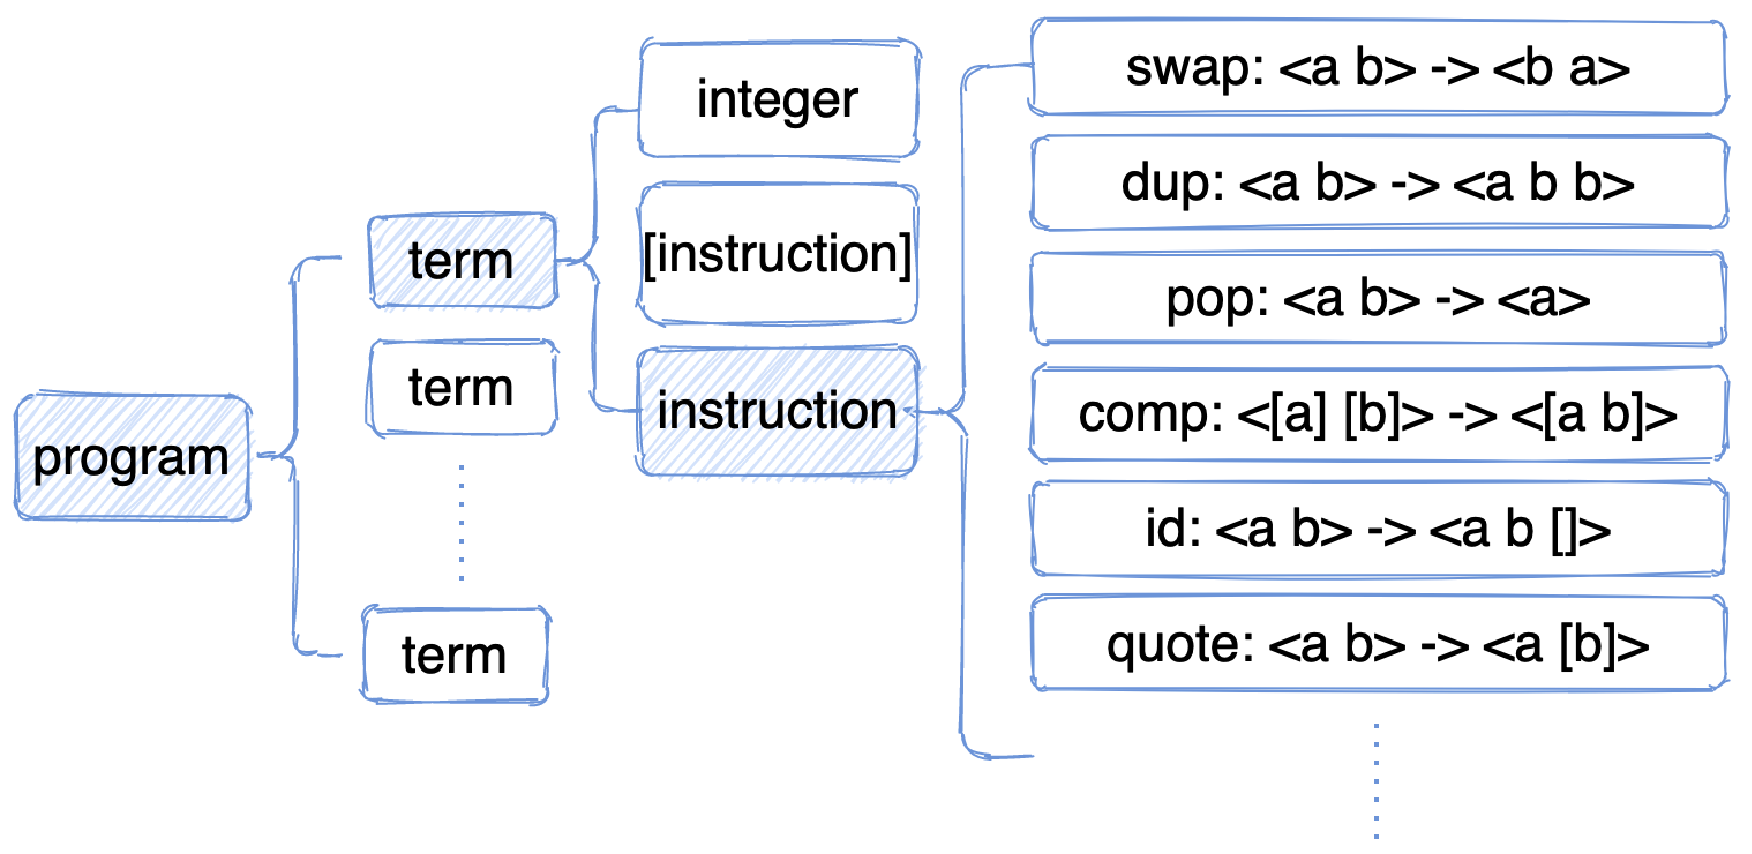
\includegraphics[width=0.8\textwidth]{syntax.pdf}
    \caption{Syntax}
    \label{fig:syntax}
\end{figure}

There are many advantages of our language. Firstly, it is statically typed which means it is easy to filter out bad programs. Secondly, it does not have variables, there is only a list of operations where every operation can manipulate the global stack. Each operation is either a command or a value. All commands in this DSL are functions that take a stack as input, and return a new stack as output. This feature makes the language easy to be generated and encoded, this serves as a great advantage regarding the program synthesis task. Due to the linearity of this language, it is easier to use beam search on it than on other languages. Lastly, in support of higher-order functions, we have a special expression form - quotation. It is a unary constructor, an instruction can be turned into a value by quoting, then it can be pushed into the global stack and applied later. In our DSL the quotation of a program is written by enclosing it in square brackets.

Here is an example: given input stack $<3,5,1>$ and program $[swap, pop, mul]$, assuming the leftmost is the top of the stack. 
\begin{DispWithArrows*}
    &<3, 5, 1> \Arrow{Swap} \\
    &<5, 3, 1> \Arrow{Pop} \\
    &<3, 1> \Arrow{Dup} \\
    &<3, 3, 1> \Arrow{Mul}\\
    &<9, 1> 
\end{DispWithArrows*}

In the end, we have 9, 1 in the resulting stack.

\subsection{Descriptions of stack-based concatenative language}
\label{sec:lang}
During the animated demonstration, you may encounter the following instructions, below are some detailed explanations. 
\begin{description}[labelwidth = 3em, leftmargin = !]
    \item[Swap] For a stack with at least two items, interchange the top two elements.
    \item[Dup] For a stack with at least one item, duplicate the topmost element on the stack.
    \item[Pop] For a stack with at least one item, remove the topmost element from the stack.
    \item[Comp] For a stack with two quoted programs on the top, replace them with a new quotation that is the result of composing the top quotation with the second quotation.
    \item[Id] For any stack, push a quoted identity program to the stack.
    \item[Quote] For a stack with at least one item, turn an integer or an instruction to quotation form. 
    \item[Apply] For a stack with at least one quotation, apply takes the top quoted program, and applies it to the rest of the stack.
    \item[Dip] For a stack with at least one quotation, apply the quoted program under the top most element to the rest of the stack.
    \item[Add] For a stack with at least two integers, add the top two integers.
    \item[Sub] For a stack with at least two integers, subtract the Second integer from the first integer.
    \item[Mul] For a stack with at least two integers, multiply the top two integers.
    \item[Div] For a stack with at least two integers, divide the Second integer with the first integer.
    \item[Mod] For a stack with at least two integers, get the remainder of the second integer divided by the first integer.
\end{description}

\noindent Overall, our DSL contains:
\begin{itemize}
    \item First-order instructions Swap, Dup, Pop, Comp, Id, Quote, Apply, Dip.
    \item Integer instructions Add, Sub, Mul, Div, Mod.
\end{itemize}
By converting them into quotation form, we can use them as higher-order commands.


\section{Using}
\label{using}
\subsection{System functions}

After successfully running the program, you will see the following main screen. It has a brief description of the software and some instructions to the user.
\begin{figure}[H]
    \centering
    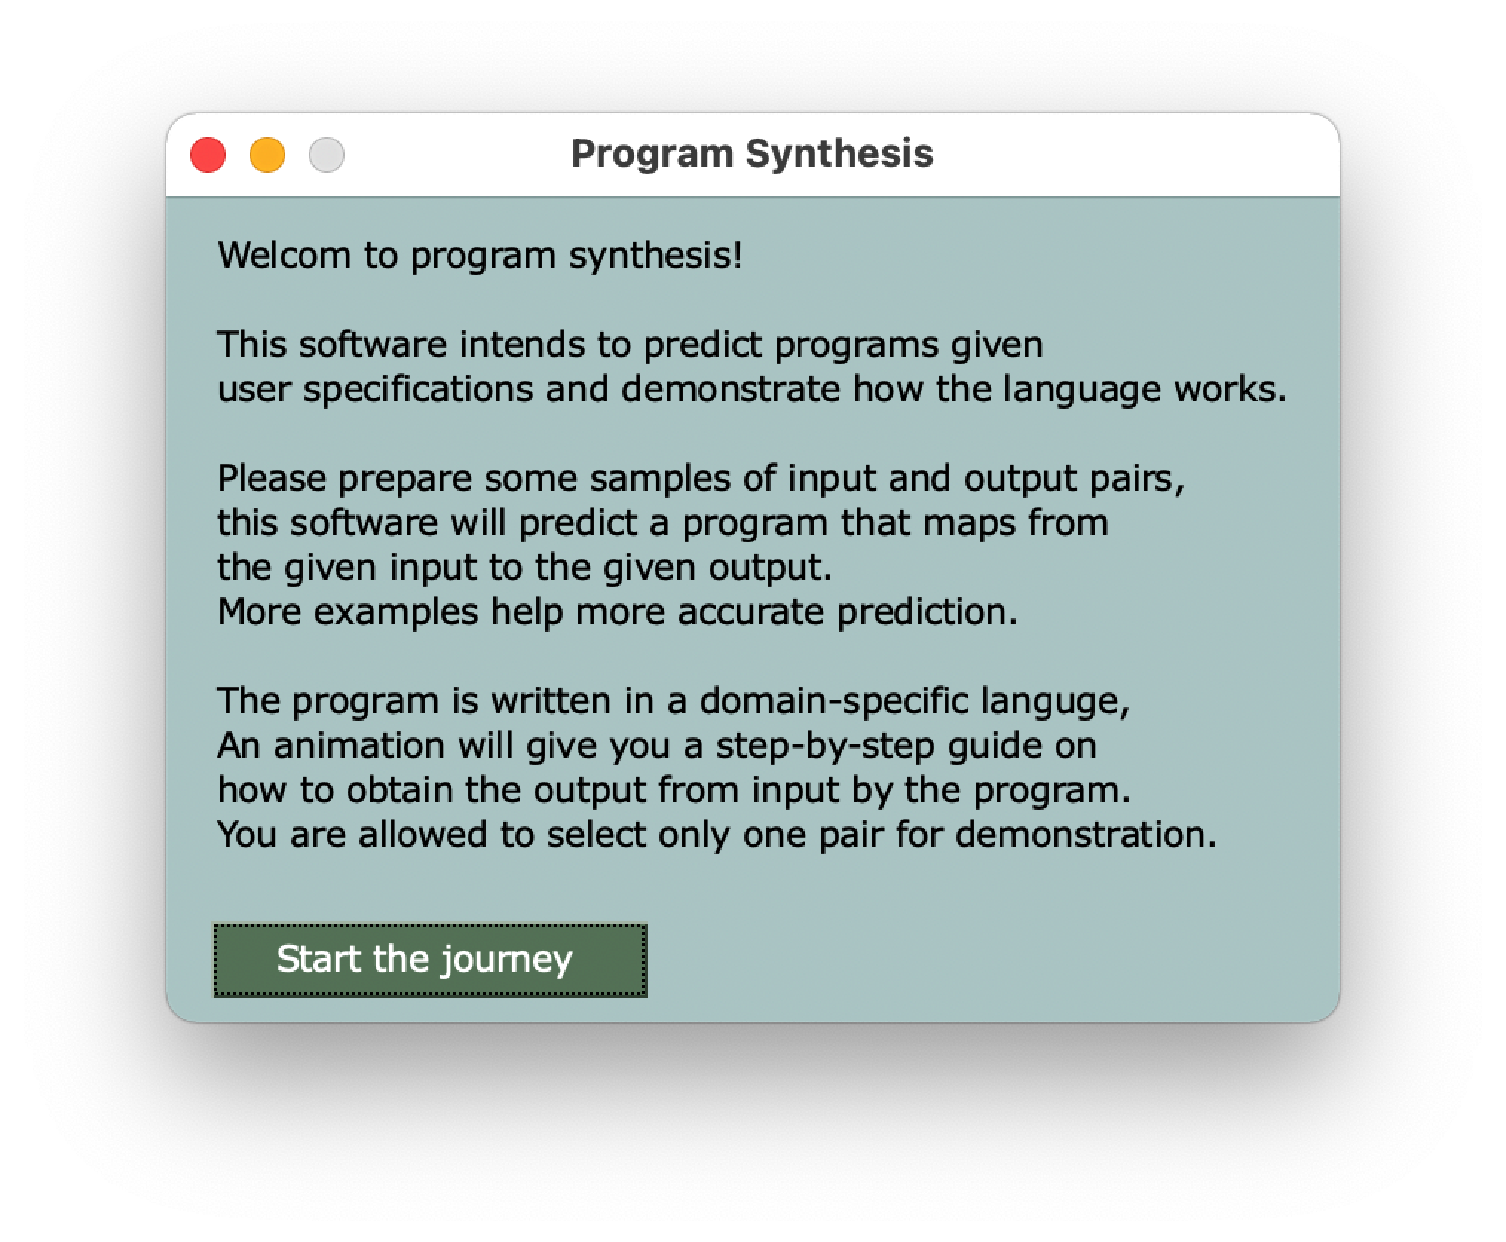
\includegraphics[width=0.55\textwidth]{start.pdf}
	\caption{Main screen}
	\label{fig:main screen}
\end{figure}

The button leads to the window of user specification (Figure \ref{fig:user specification}), you can type the number of input and output pairs that you want to give. These pairs will later be sent to the beam search algorithm to make the prediction and one of them will be selected for demonstration.

\begin{figure}[H]
    \centering
    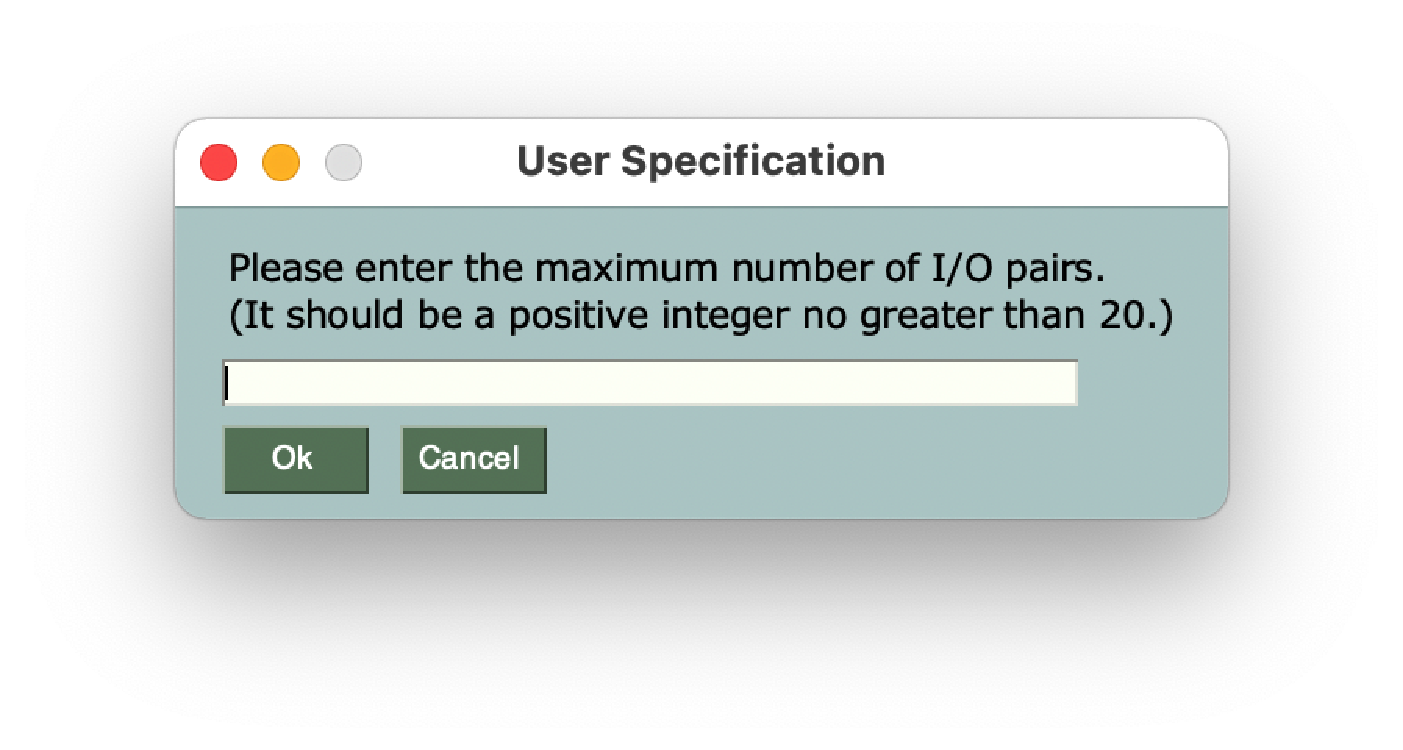
\includegraphics[width=0.55\textwidth]{pairs.pdf}
	\caption{User Specification}
	\label{fig:user specification}
\end{figure}

Then you will be redirected to another window for entering concrete samples. You need to pay attention to the requirements written in the windows box, if you give illegal values, you will get error messages(We will discuss this later in Section \ref{messages}). For example it is six in this case (see Figure \ref{fig:user specification}).

\begin{figure}[H]
    \centering
    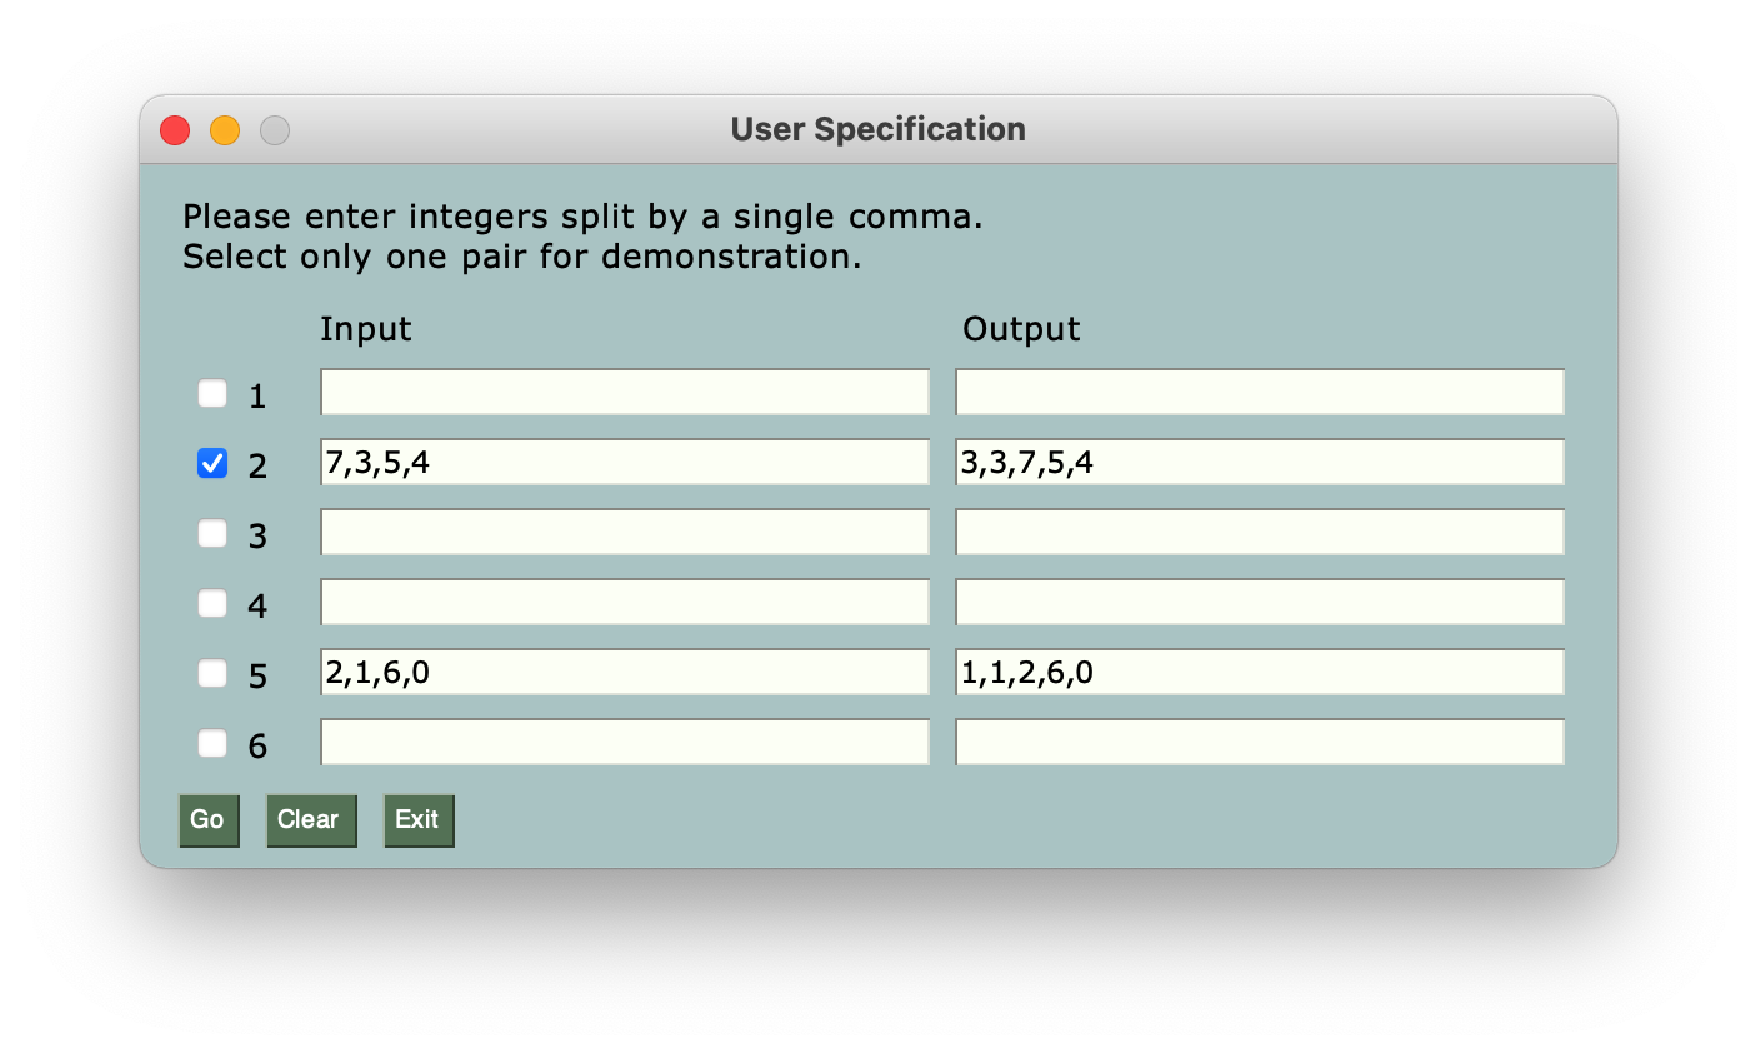
\includegraphics[width=0.6\textwidth]{input.pdf}
	\caption{User Input}
	\label{fig:user input}
\end{figure}

By clicking the ``Ok" button, you will be redirected to another window. Here the user needs to enter at least one pair and at most six pairs of input and output examples. More pairs provide the model with more information, so the result will be more accurate. After finishing the input, you need to choose only one pair among what you have typed for demonstration purpose (as shown in Figure \ref{fig:user input}).
\begin{wrapfigure}{l}{0.45\textwidth}
    \centering
    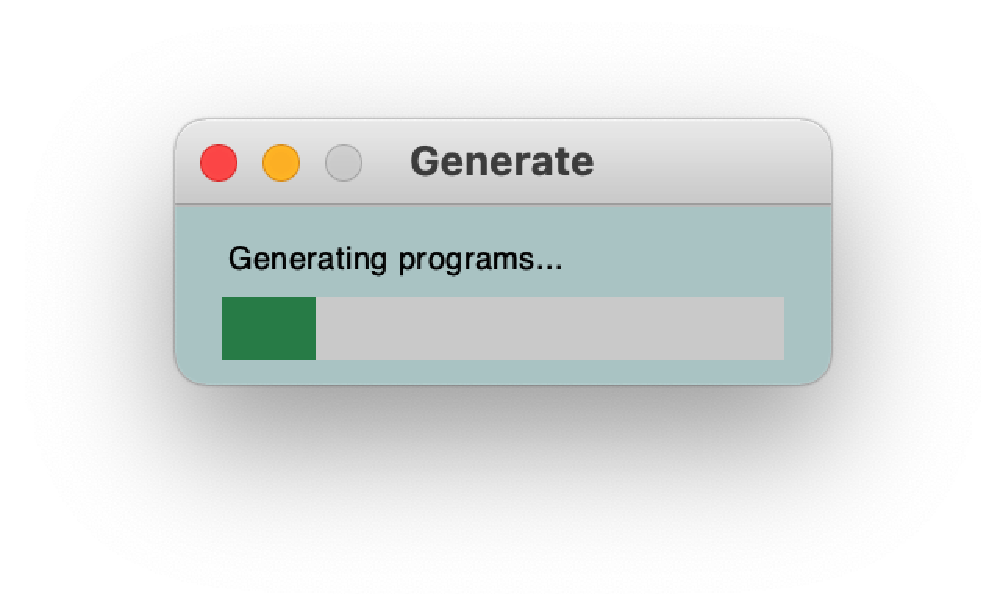
\includegraphics[width=0.4\textwidth]{progress_bar.pdf}
	\caption{Progress Bar}
	\label{fig:progress bar}
\end{wrapfigure}
After specifying all the needed information, the model will work on generating the program to satisfy user input, you will see a screen similar to Figure \ref{fig:progress bar}. The maximum length of the progress bar is set to equal to the max depth of beam search. It is possible that the suitable program is found before the searching reach the deepest level. Therefore, the screen may end before the progress bar reaches the end. 

When beam search gets the desired program, you will the the screen as Figure \ref{fig:demonstrate} shows. On the top of the main screen displays the instructions that can finish the given task. The stack below it starts with the initial state and will change according to the instruction. User can click the ``Next'' button to see how each step works and how the stack changes to go from the input to output with the generated instructions. And the checkbox can be used to hide or show the user input.

\begin{figure}[H]
  \centering
  \begin{minipage}[b]{0.43\textwidth}
    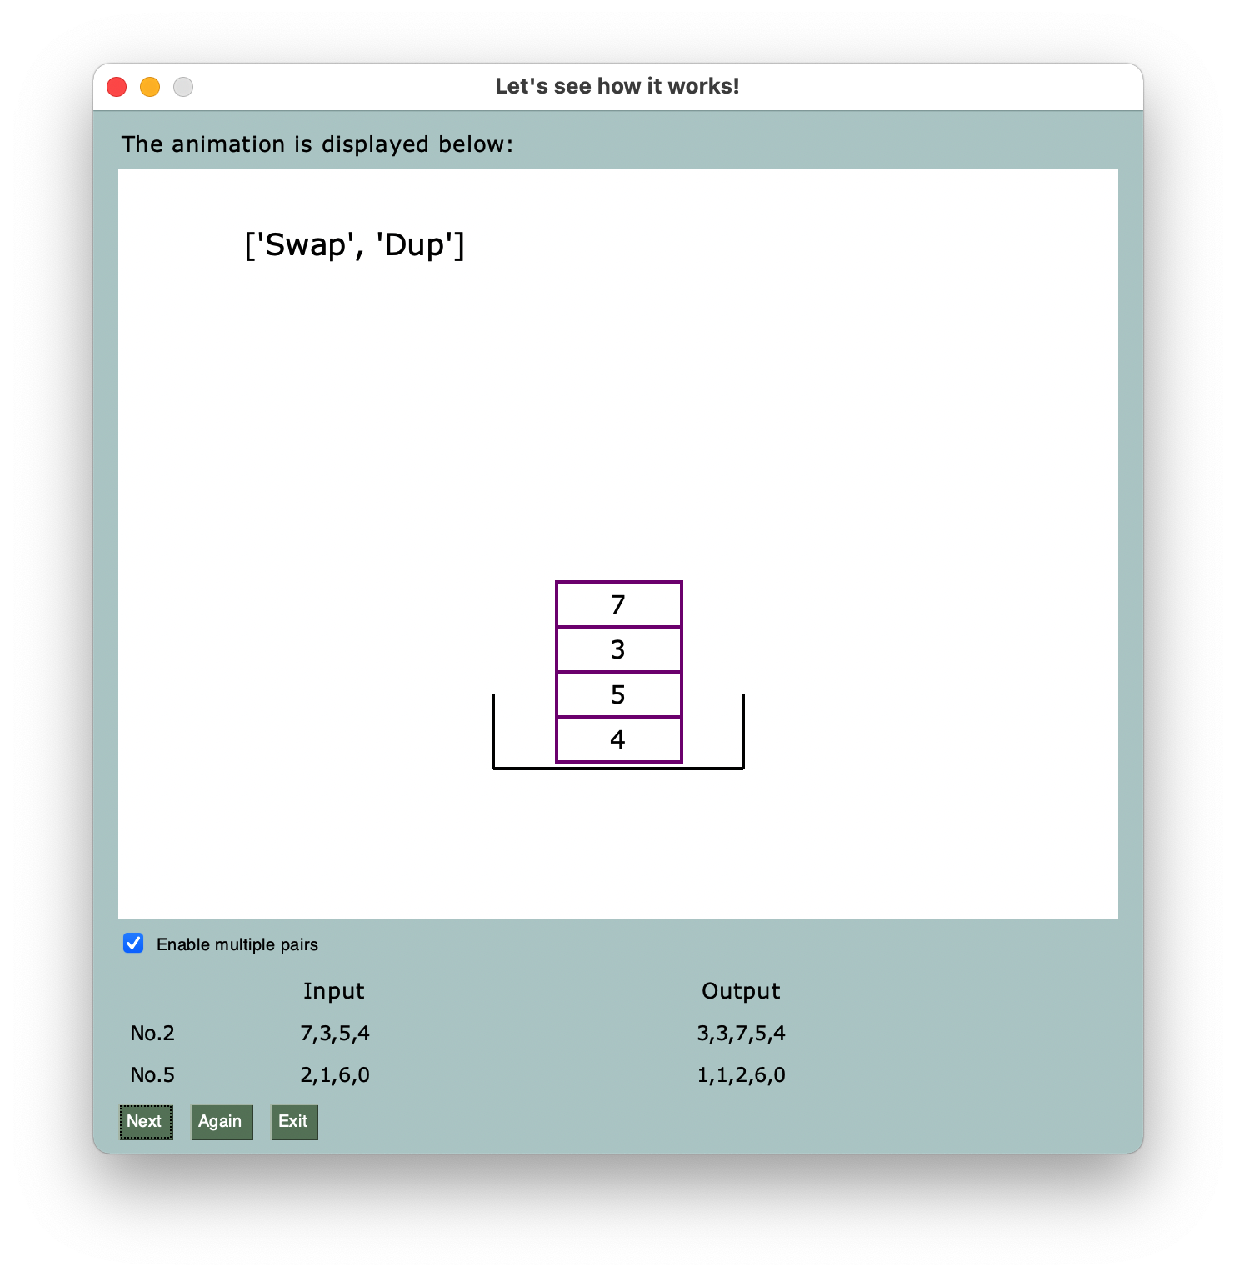
\includegraphics[width=\textwidth]{demonstrate.pdf}
    \caption{Demonstration screen}
    \label{fig:demonstrate}
  \end{minipage}
  \hfill
  \begin{minipage}[b]{0.43\textwidth}
    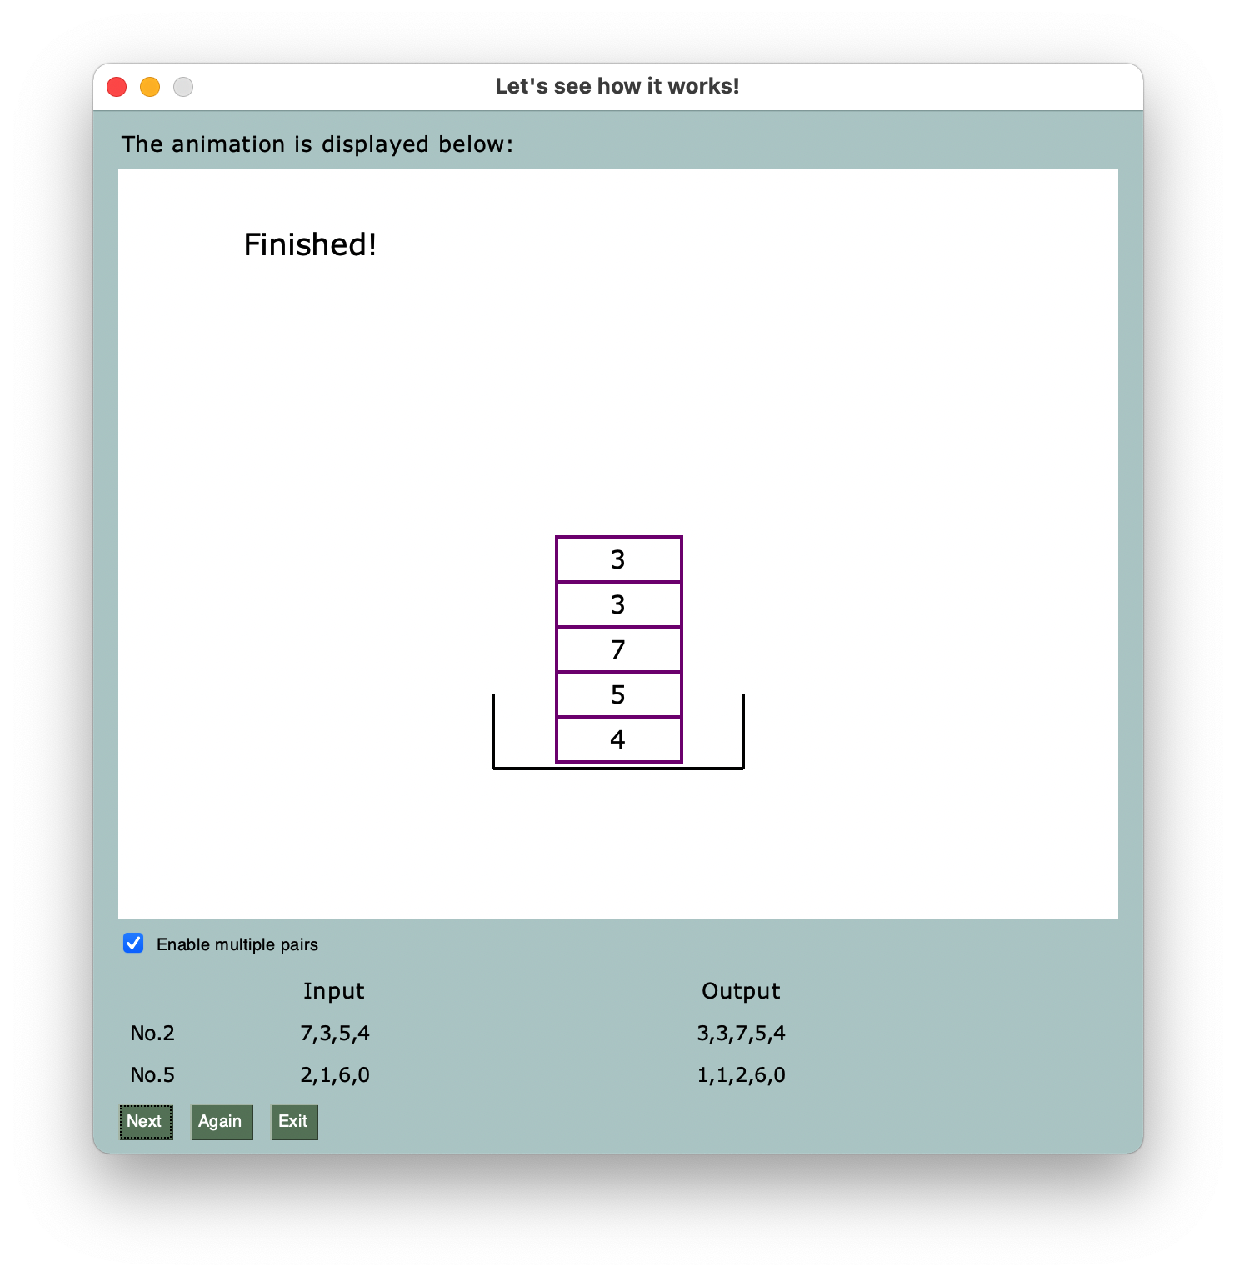
\includegraphics[width=\textwidth]{finish.pdf}
    \caption{Finish screen}
    \label{fig:finish}
  \end{minipage}
\end{figure}

If the search ends, but no program is found, then the user can try again with other input and output pairs.

\subsection{Run-time system messages}
\label{messages}
At the beginning, when the user is required to give a maximum number for input and output pairs, if they press the ``Ok" button without entering an integer or entering other illegal characters which do not meet the requirement of the description, they may get the following error messages.

\begin{figure}[H]
  \centering
  \begin{minipage}[b]{0.28\textwidth}
    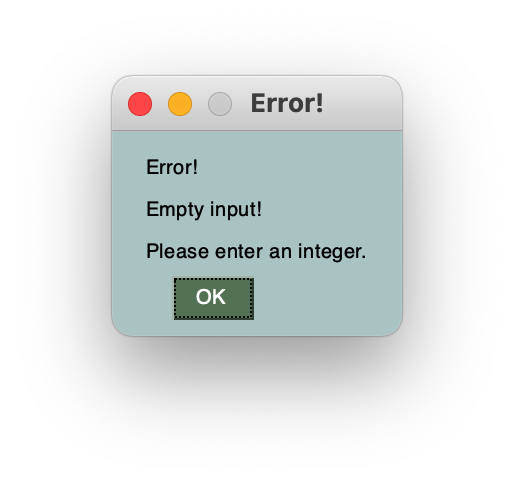
\includegraphics[width=\textwidth]{input_pair_errors/empty_pair.png}
    \caption{Error message for empty input}
  \end{minipage}
  \hfill
  \begin{minipage}[b]{0.29\textwidth}
    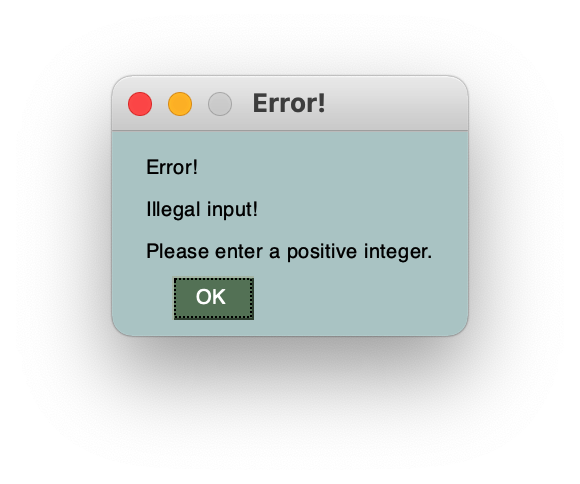
\includegraphics[width=\textwidth]{input_pair_errors/negative_pair.png}
    \caption{Error message for negative numbers}
  \end{minipage}
  \hfill
  \begin{minipage}[b]{0.3\textwidth}
    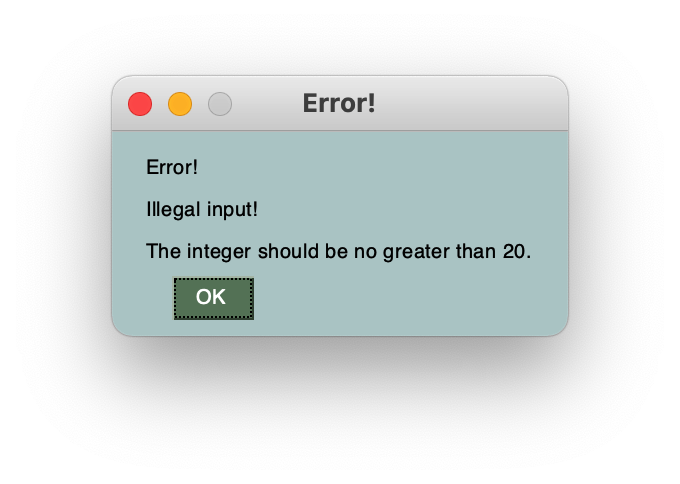
\includegraphics[width=\textwidth]{input_pair_errors/large_pair.png}
    \caption{Error message for large numbers}
  \end{minipage}
\end{figure}

After specifying the custom I/O pairs, the user needs to tick one checkbox for demonstration. They may get the following error messages if:
\begin{itemize}
    \item They forget to select one pair to demonstrate. See Figure \ref{error1}.
    \item They select more than one pair. See Figure \ref{error2}.
\end{itemize}

\begin{figure}[H]
  \centering
  \begin{minipage}[b]{0.4\textwidth}
    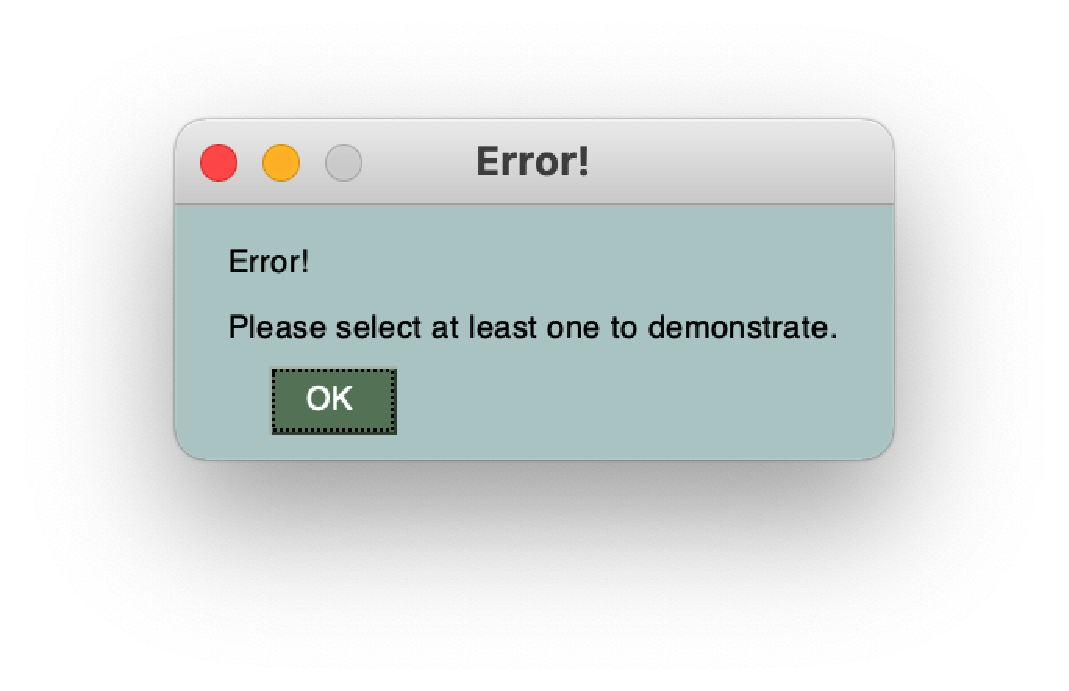
\includegraphics[width=\textwidth]{error1.pdf}
    \caption{Error message for not selecting}
    \label{error1}
  \end{minipage}
  \hfill
  \begin{minipage}[b]{0.4\textwidth}
    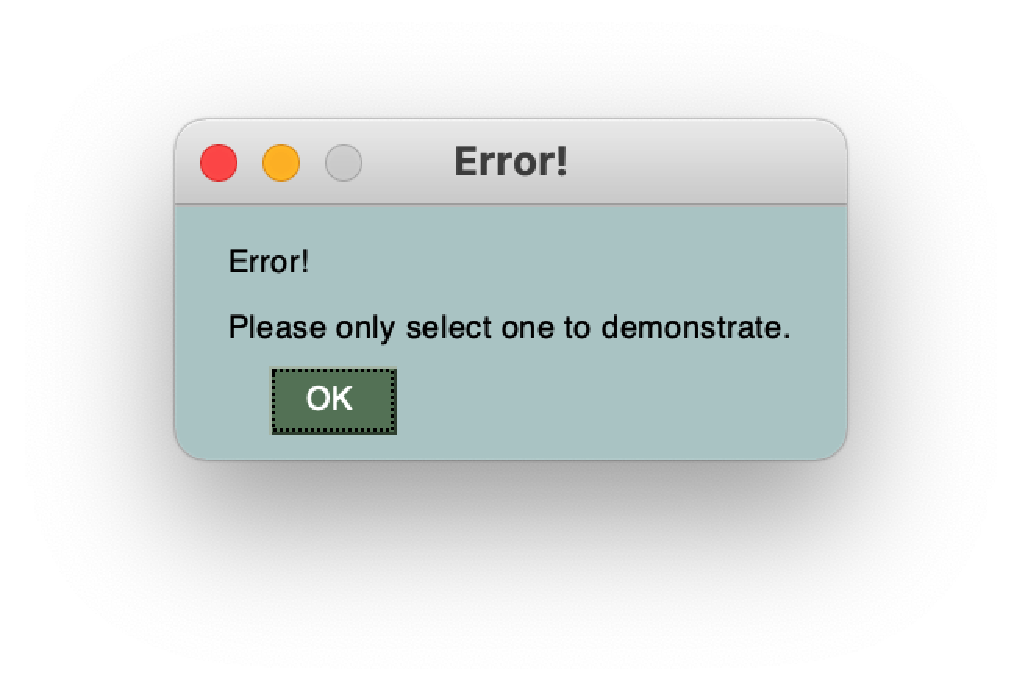
\includegraphics[width=\textwidth]{error2.pdf}
    \caption{Error message for multiple selecting}
    \label{error2}
  \end{minipage}
\end{figure}
\chapter{Developer Documentation}
\label{dev}
\section{Overview}
\label{sec:overview}
\subsection{File structure}
\dirtree{%
    .1 /stack-prog-synth.
    .2 stackprogsynth.
    .3 data.
    .3 gui.
    .3 lang.
    .3 nn.
    .3 beamSearch.py.
    .3 constants.py.
    .3 utils.py.
    .2 tests.
    .3 data.
    .3 lang.
    .3 test\_utils.py.
    .2 environment.yml.
    .2 gen.py.
    .2 main.py.
    .2 train.py.
    .2 treelstm.pyi.
}

The tree above shows the file structure of the whole project. This is a joint work of a fellow student Xie Zongpu and me. 

\texttt{stack-prog-synth} is the project folder and \texttt{stackprogsynth} is the source folder, the following was written by me:
\begin{enumerate}
    \item \texttt{lang} folder, except \texttt{type.py}: for data generation, encoding, and program evaluation.
    \item \texttt{nn} folder, except \texttt{data.py}: for building the model and measuring the accuracy.
    \item \texttt{gui} folder and \texttt{main.py} file: for graphical user interface.
    \item \texttt{constants.py} file: storing constant parameters for synthetic data generation and network construction. 
\end{enumerate}

The figure below shows the dependencies of files on my part. \texttt{main.py} is in the root folder \texttt{stack-prog-synth} while all other paths are relative to the source folder which is \texttt{stackprogsynth}. The file \texttt{beamSearch.py} was written by my colleague, however, it is necessary to be included in the figure since this part serves as an important bond between different modules.
\begin{figure}[H]
    \centering
    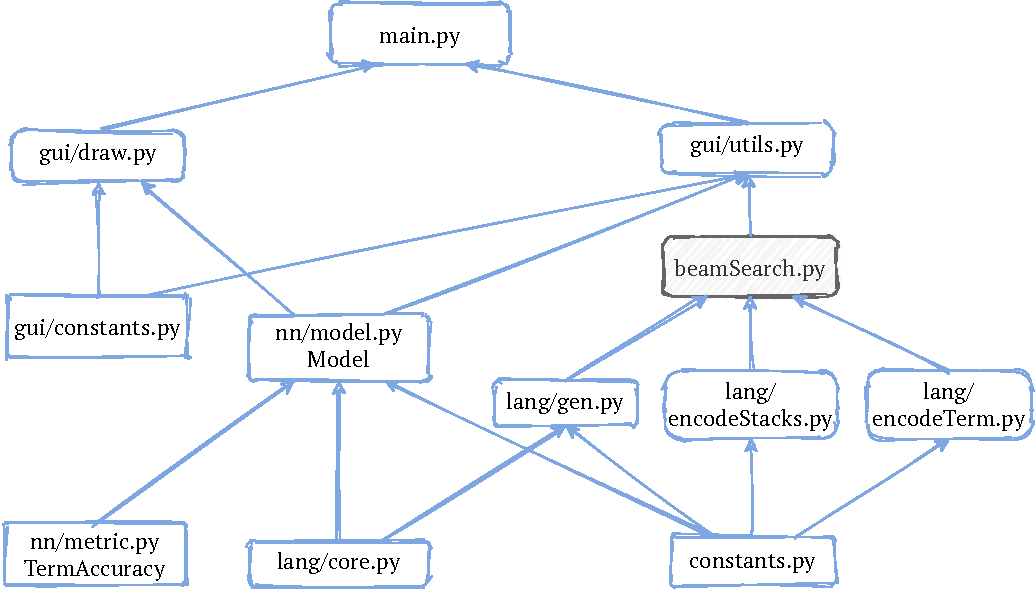
\includegraphics[width=1.0\textwidth]{dependencies.pdf}
    \caption{Dependencies of modules}
    \label{fig:dep}
\end{figure}
The next session will give a brief summary of each module and the following sections will explain the implementation of each part in detail.

\subsection{Software architecture}
Figure \ref{fig:uml} is the class diagram that covers most part of the project. It shows the connections between separate modules. 
\begin{figure}[H]
    \centering
    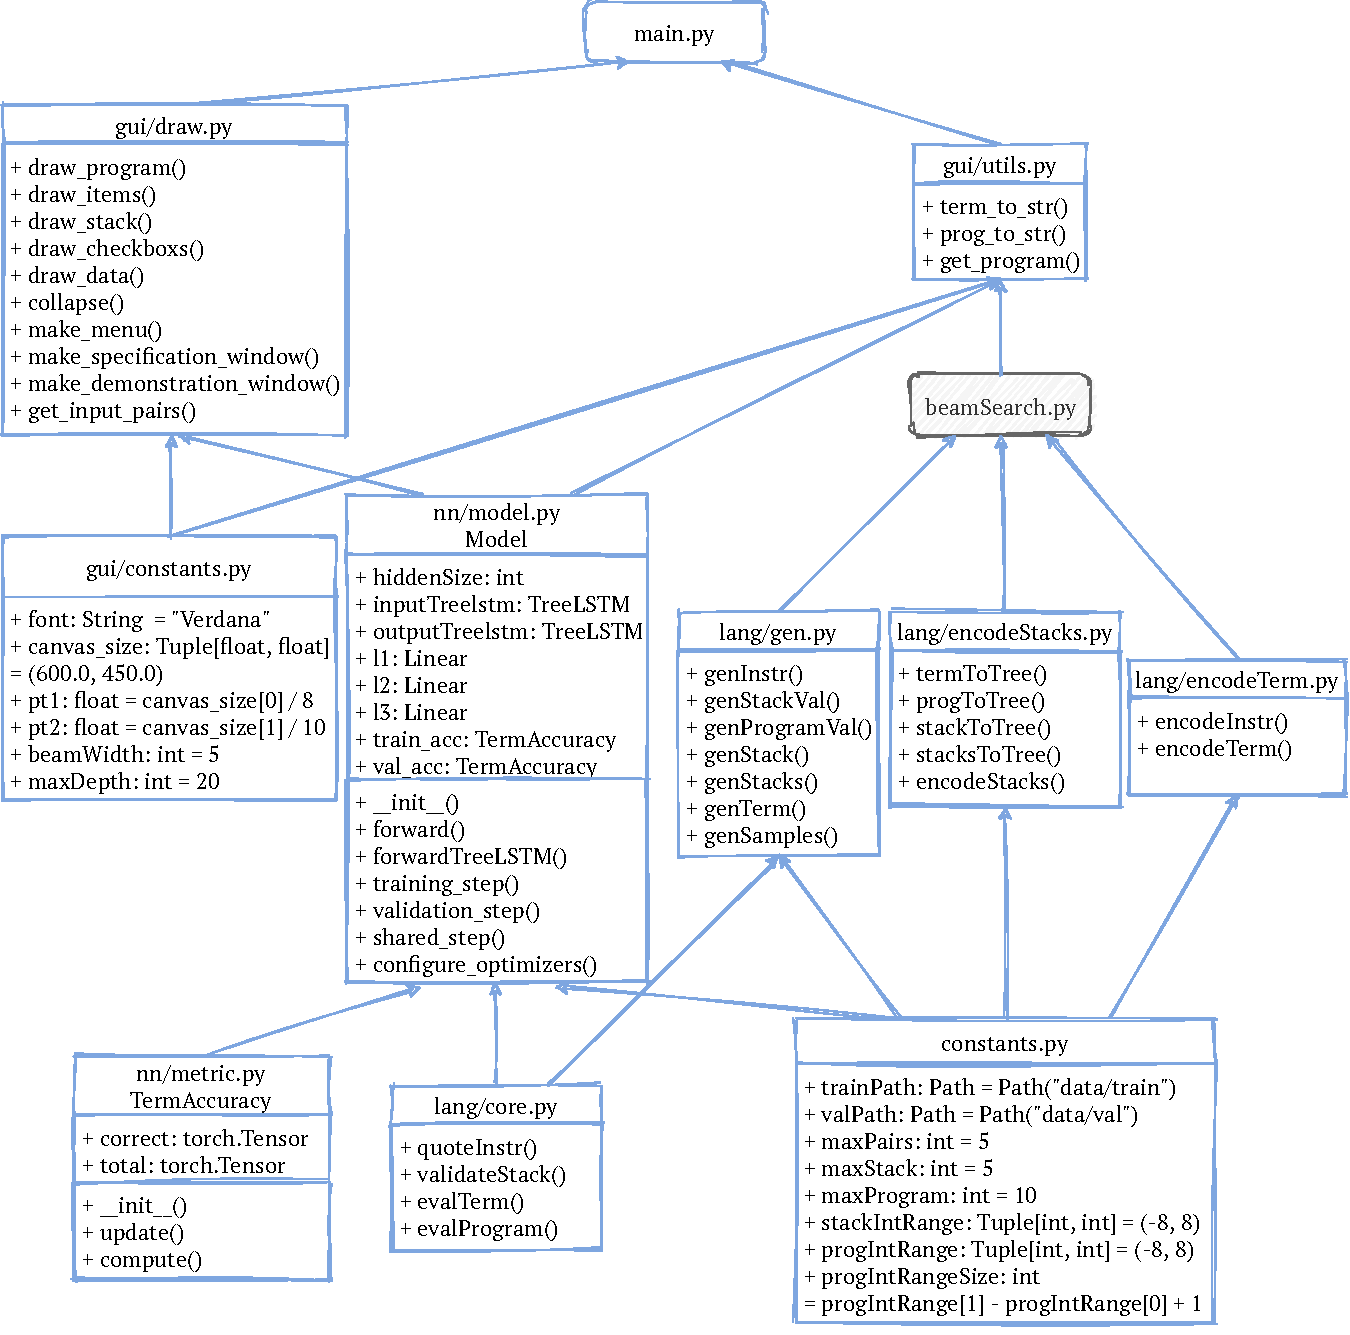
\includegraphics[width=1.05\textwidth]{UML.pdf}
     \caption[Connections between different modules; (function parameters and return types are omitted)]
    {\tabular[t]{@{}l@{}}Connections between different modules \\ (function parameters and return types are omitted)\endtabular}
    \label{fig:uml}
\end{figure}
To start with, the user can run \texttt{main.py} to start the program. It has the main function that uses PySimpleGUI \cite{psgui} to render windows and handle events. Coordinating with \texttt{draw.py} and \texttt{utils.py}, it is able to pass user input to the beam search algorithm and get the predicted result.

File \texttt{draw.py} offers functions for stack animations and layout design. In \texttt{utils.py}, \texttt{get\_program} will give trained model to \texttt{beamSearch} to obtain the prediction, and \texttt{prog\_to\_str} will convert the program to string so that it can be displayed in the window.  \texttt{constants.py} in \texttt{gui} folder has constant parameters for rendering the window and using the beam search algorithm.

\texttt{model.py} has the class \texttt{Model}. It inherits \texttt{LightningModule} from the PyTorch Lightning \cite{pytorch-ligntning} library. This custom class has methods to build the network, create Tree-LSTM and linear layer, and train the model. It also has instances of \texttt{TermAccuracy} to measure the performance of the prediction.

\texttt{gen.py} is used for synthetic data generation, this will be discussed in detail in Section \ref{sec:datagen}. Files \texttt{encodeStack.py} and \texttt{encodeTerm.py} are used to convert data structures to tree then encode them, so that the Tree-LSTM layer can be applied. Section \ref{sec:encoding} will talk more about this.

The file \texttt{core.py}, as the name suggests, contains the core of the language. It implements the stack-based concatenative languge, see details in Section \ref{sec:impdsl}. The evaluation functions \texttt{evalTerm} and \texttt{evalProgram} are used to get the target result from the input. \texttt{validateStack} checks the integer ranges in the stack and \texttt{quoteInstr} converts an instruction to a quotation.

In the root folder, \texttt{constants.py} defines constant arguments for data synthesis and layer creation. It contains integer ranges that are used by the encoding files for validation. And the stack size and program length are used by \texttt{gen.py} for generating stack values and programs.

\subsection{General workflow}
The following figure gives an overview of the whole project. The part inside the rectangle is the architecture of our neural network, and this will be discussed in Section \ref{sec:network}.

Generally speaking, we generate random input stacks and programs, by running the evaluation function \texttt{evalProgram} in \texttt{core.py}, we can get the corresponding output stacks. We then encode the input and output stacks and feed them into the Tree-LSTM neural network. Using supervised learning, we encoded the desired output program at the same time and compare it with the result that is given by the model. After this, the neural network will calculate the loss and the Adam optimizer \cite{adamW} will make mini-batch gradient descent and back-propagation \cite{BP}, repeat the training process until the model reaches a decent validation accuracy. 

When the model is prepared, we can use beam search on it to predict terms. Given input and output pairs, our trained model will give a probability for each term. The beam search algorithm then will rank the scores and find the most suitable fit as a solution.
\begin{figure}[H]
    \centering
    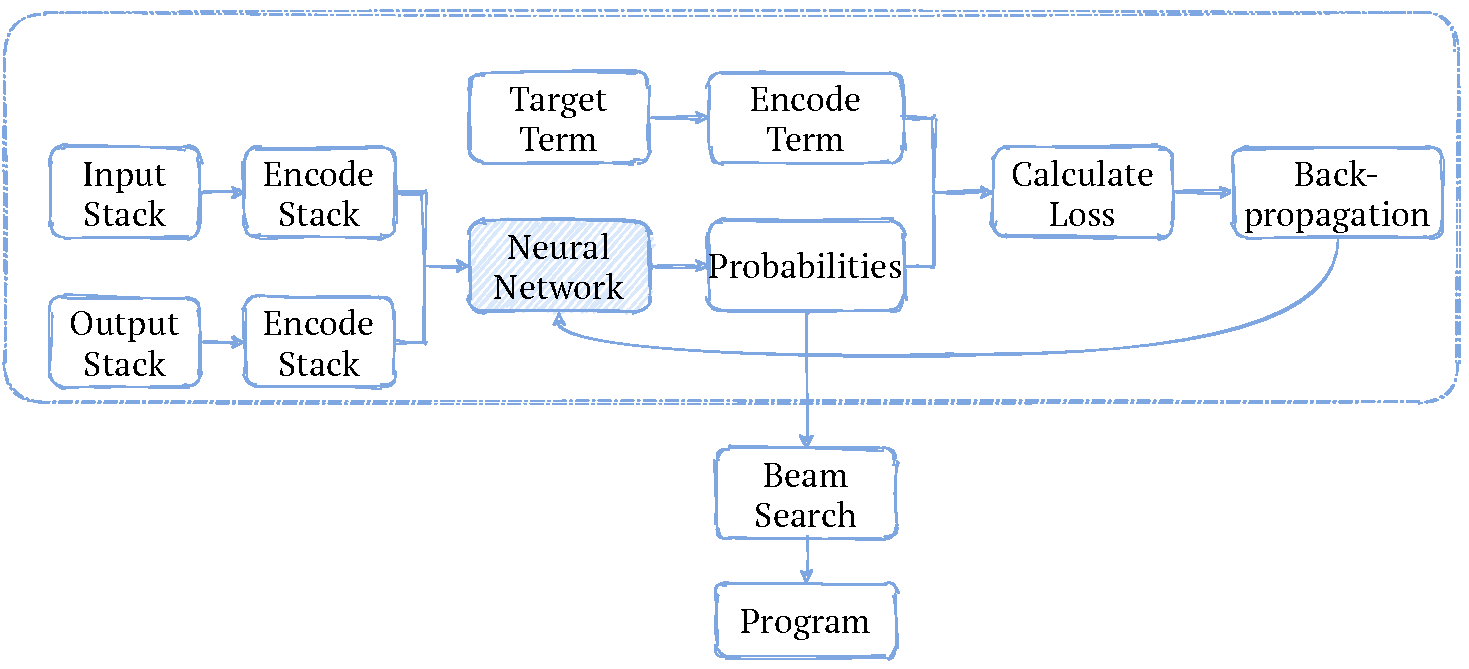
\includegraphics[width=0.85\textwidth]{workflow.pdf}
    \caption{Workflow}
    \label{fig:workflow}
\end{figure} 

\section{DSL in Implementation}
\label{sec:impdsl}
The following shows the UML for implementation of the stack-based concatenative language. 

\texttt{Instr}, \texttt{Val}, \texttt{Int} and \texttt{Quoted} are classes for the ADT constructor. \texttt{Term}, \texttt{Program}, \texttt{Instruction} and \texttt{Value} are type synonyms, with \texttt{Term} defined as \texttt{T.Union[Instr, Val]}, \texttt{Instruction} defined as \texttt{T.Union[
    Swap, Dup, Pop, Comp, Id, Quote, Apply, Dip, Add, Sub, Mul, Div, Mod
]} and \texttt{Value} defined as \texttt{T.Union[Quoted, Int]}.

Type \texttt{Union} in the typing module \cite{typing} was used to in the procedure. \texttt{Union[X, Y]} mean either X or Y. Similar to inheritance \cite{wiki:inheritance} in object-oriented programming \cite{wiki:oop}, it represents subtypes from base types. However, it is closed for extensions \cite{wiki:open-closed}.

\texttt{Program} is the type synonym of \texttt{Deque[Term]}. The abstract data type \texttt{Deque} gives back a new object instead of changing the original. This makes programs more efficient to manipulate persistently, meaning it allows access to any version, old or new, at any time \cite{driscoll1989making}. When using the beam search algorithm, we need to be able to append to one version of the structure in multiple ways so as to check different possible terms.

\begin{figure}[H]
    \centering
    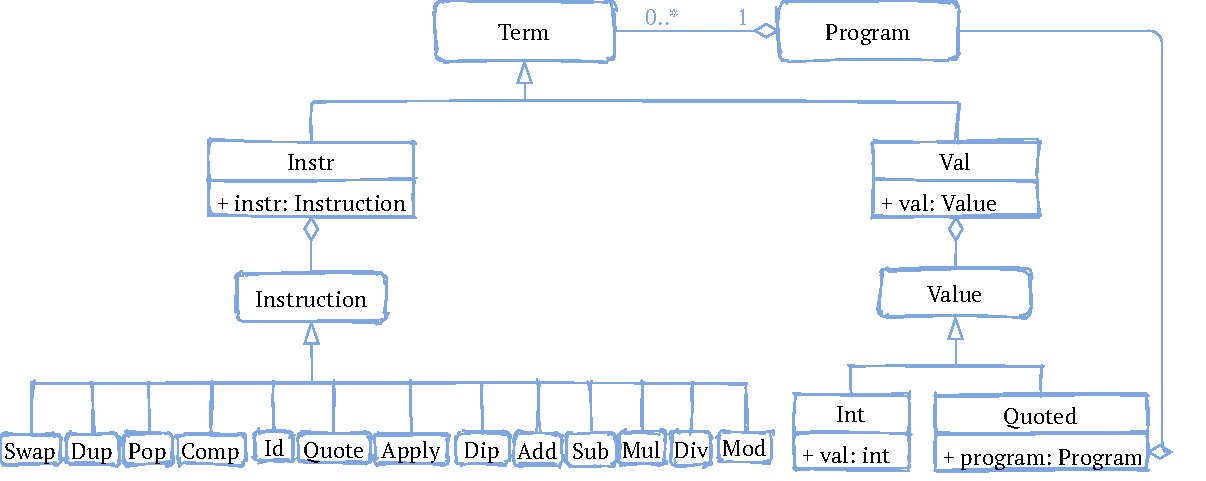
\includegraphics[width=\textwidth]{UML-Lang.pdf}
    \caption{Class diagram of the stack language AST}
    \label{fig:uml-lang}
\end{figure}

Section \ref{sec:lang} has a detailed description of each instruction and \texttt{evalTerm} implements the functionalities of each of them. Values are pushed to the stack. Integer operations \texttt{Add}, \texttt{Sub}, \texttt{Mul}, \texttt{Div} and \texttt{Mod} expect two integer values on the top of the stack. Some functions expect quoted programs on top of the stack and execute them in many different ways, effectively by dequoting, examples are \texttt{Apply} and \texttt{Dip}. The code below shows a small part of evaluating a term on a stack in \texttt{evalTerm} function.

\begin{listing}[H]
\begin{minted}{python}
        if isinstance(term.instr, Comp):
            fst, stack = stack.pop()
            snd, stack = stack.pop()
            if isinstance(fst, Quoted) and isinstance(snd, Quoted):
                return stack.push(Quoted(deque(snd.program + fst.program)))
            raise ValueError(fst, snd)
        if isinstance(term.instr, Id):
            return stack.push(Quoted(deque()))
        if isinstance(term.instr, Quote):
            value, stack = stack.pop()
            return stack.push(Quoted(deque([Val(value)])))
\end{minted}
\caption{Implementation of Comp, Id, and Quote}
\end{listing}

\section{Data Processing}
\label{sec:datagen}
\subsection{Synthetic data generation}
Synthetic data is artificial data generated to preserve privacy, testing systems, or creating training data for machine learning algorithms. 
Synthetic data generation is critical since it is an important factor in the quality of synthetic data \cite{synthdata}. 
If one does not have clean and well-prepared data, they may encounter garbage in, garbage out situations. Besides, the performance of a machine learning model is upper bounded by the quality of the data \cite{dataquality}. Therefore, generating enough amount of data with good quality is not only a prerequisite but also one of the requirements for a successful model training.

For our project, we need to generate stacks and programs separately. We treated a tuple of an input stack and a term and the resulting stack as one sample. Figure \ref{fig:gen} illustrates the functions we wrote for synthesizing data and the relationship between them. And here follows how we generated samples in detail. 

\begin{wrapfigure}{l}{0.5\textwidth}
    \centering
    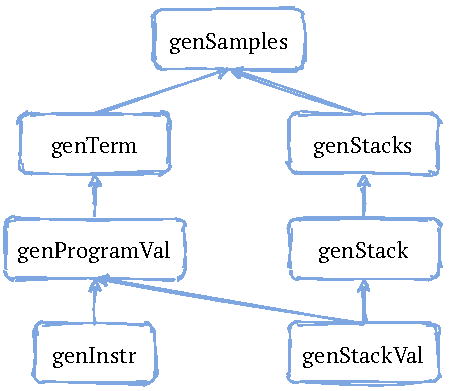
\includegraphics[width=0.5\textwidth]{gen.pdf}
    \caption{Functions for data generation}
    \label{fig:gen}
\end{wrapfigure}

For programs, we have \texttt{genProgramVal} which creates random integer values in a predetermined range and uses \texttt{genInstr} to generate instructions. The \texttt{genTerm} function gets a random stack, returns a tuple of a generated term, and a tuple of new stacks. It will prune away invalid stacks or redundant programs. 

For stacks, \texttt{genStack} uses \texttt{genStackVal} to get random integer values within a certain bound, for the sake of simplicity, we now only allow input stacks to have integers. \texttt{genStacks} returns a tuple that contains \texttt{maxPairs} of stacks, and each stack has a length that equals to \texttt{maxStack}. Finally, \texttt{genSamples} (see Listing \ref{fun:genSamples}) uses \texttt{genTerm}  and \texttt{genStacks} to return a list of samples. \texttt{genTerm} checks the type of the new term and the elements in the new stacks. \texttt{genSamples} managed to avoid repetition of stacks in the resulting list.

\begin{listing}[H]
\begin{minted}{python}
def genSamples(
    rng: Random = Random(),
) -> T.List[T.Tuple[T.Tuple[Stack[Value], ...], T.Tuple[Stack[Value], ...], Term]]:
    samples: T.List[T.Tuple[T.Tuple[Stack[Value], ...], Term]] = []
    currStacks = genStacks(rng)
    inStacks = currStacks
    progNum = rng.randint(1, maxProgram)
    result = {currStacks}

    for _ in range(progNum):
        newTerm, newStacks = genTerm(inStacks, rng)
        if newStacks not in result:
            result.add(newStacks)
            samples.append((currStacks, newTerm))
            currStacks = newStacks
    return [(inp, currStacks, newTerm) for (inp, newTerm) in samples]
\end{minted}
\caption{genSamples function}
\label{fun:genSamples}
\end{listing}

It is important to note in advance that integers are infinite, we have to set bound to them in order to do the encoding before passing them to the neural network. All the predetermined ranges are written in \texttt{constants.py} file. We set the range of integers in the program from -8 to 8, since small numbers are more frequent and a program with small numbers can manipulate big numbers. The file also defines the maximum size of a stack and the maximum allowed number of input-output pairs in a stack. These settings will not restrict our program to a large extent since integers can always get bigger numbers by adding or multiplying and stacks can expand. 
\subsection{Abstract syntax tree embedding}
\label{sec:ast}
By having quotations in our stacks, they can have programs as first-class functions, which makes them not linear structures anymore. As a result, we need to look for neural networks that are suitable for tree-structured inputs instead of using the conventional recurrent neural network which is for linear data. We decided to use Tree-structured Long Short-Term Memory \cite{tree-lstm} networks to deal with non-linearity. Tree-LSTM is a generalization of LSTM which works on tree-structured inputs. We used a Python library \texttt{pytorch-tree-lstm} \cite{pytorch-tree-lstm}. It is an implementation of the child sum Tree-LSTM model \cite{tree-lstm}, and it supports vectorized tree evaluation and batching.
\begin{figure}[H]
    \centering
    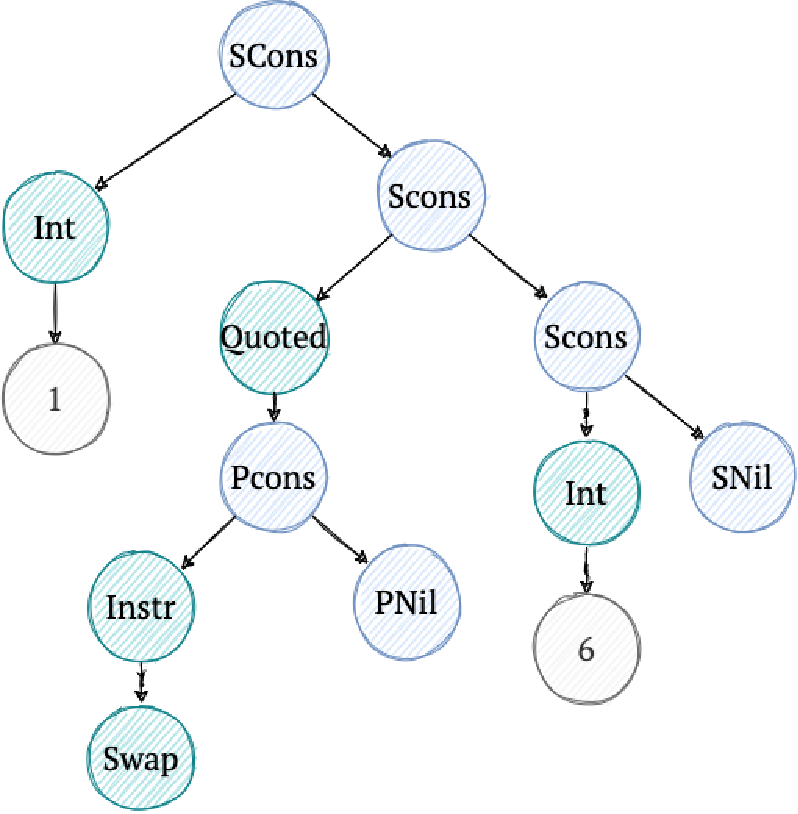
\includegraphics[width=0.5\textwidth]{tree.pdf}
    \caption{Abstract syntax tree}
    \label{fig:tree}
\end{figure}
First, we need to convert stacks to trees. As the example shown in Figure \ref{fig:tree}, by having constructors like SCons, SNil, PNil, Quoted (they are stored in \texttt{labelClasses}, see Listing \ref{labels}), we can turn the stack $<Int(1), Quoted([Instr(Swap)]), Int(6)>$ to a tree. Then, with the help of the library, we are able to convert each node to a tensor so that it can be given to the Tree-LSTM structure.  

\begin{listing}[H]
\begin{minted}{python}
labelClasses: T.List[T.Union[str, int]] = (
    [
        constr.__name__
        for constr in T.get_args(Term) + T.get_args(Value) + T.get_args(Instruction)
    ]
    + ["PCons", "PNil", "SCons", "SNil", "TCons", "TNil"]
    + [i for i in range(stackIntRange[0], stackIntRange[1] + 1)]
)
\end{minted}
\caption{labelClasses}
\label{labels}
\end{listing}

\subsection{Encoding}
\label{sec:encoding}
From Figure \ref{fig:workflow} we can deduce that it is necessary to encode stacks and target terms before training. 

\begin{wrapfigure}{r}{0.5\textwidth}
    \centering
    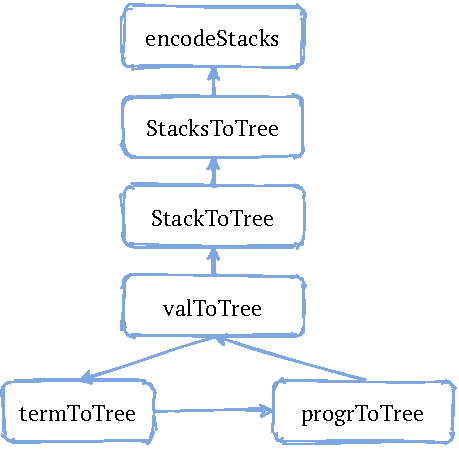
\includegraphics[width=0.5\textwidth]{encode.pdf}
    \caption{Functions for encoding stacks}
    \label{fig:encode}
\end{wrapfigure}

Figure \ref{fig:encode} exhibits the functions written for encoding stacks, the names are self-explanatory. In order to apply the Tree-LSTM layer on the stacks, it is important to first convert them to trees before encoding. As we saw in Figure \ref{fig:syntax}, programs comprise terms and terms consist of values, and quoted programs can be values. Hence, the functions \texttt{termToTree}, \texttt{progToTree} and \texttt{valToTree} are mutually recursive, it is like normal recursion where a function uses itself, they instead use each other. Mutual recursion is very common in functional programming.

The listings \ref{lst:encodeInstr} and \ref{lst:encodeTerm} are code for encoding instructions and terms. For instructions encoding, we return one plus the corresponding index of the given instruction. Since the 0th place is reserved for non-instruction types.

\begin{listing}[H]
\begin{minted}{python}
def encodeInstr(instr: Instruction) -> int:
    return T.get_args(Instruction).index(instr.__class__) + 1
\end{minted}
\caption{Function for encoding an instruction}
\label{lst:encodeInstr}
\end{listing}

\begin{listing}[H]
\begin{minted}{python}
class EncodedTerm:
    termLabel: int
    instrLabel: int
    integer: int
\end{minted}
\caption{EncodedTerm class}
\label{code:encodedTerm}
\end{listing}

\texttt{encodeTerm} returns a tuple of type \texttt{EncodedTerm}, it is a class that we created to store the encoding result, as the Listing \ref{code:encodedTerm} shows. It has three fields:
\begin{itemize}
    \item \texttt{termLabel}: Indicating the type of the new term,  0 for instructions, 1 for quotations, and 2 for integers.
    \item \texttt{instrLabel}: Specifying the type of the instruction, 0 for integers.
    \item \texttt{integer}: Representing the integer value, 0 for non-integer types and 1 to predetermined \texttt{progIntRangeSize} for integers. 
\end{itemize}

In \texttt{encodeTerm}, the \texttt{isinstance} function returns True if the specified object is of the specified type, otherwise False. We have two validations here:
\begin{itemize}
    \item Whether the quotation has only a single instruction.
    \item Whether the integer value within the predefined range.
\end{itemize}

A \texttt{ValueError} will be raised if the validation fails, otherwise, it returns an \texttt{EncodedTerm} instance.
\begin{listing}[H]
\begin{minted}{python}
def encodeTerm(term: Term) -> EncodedTerm:
    if isinstance(term, Instr):
        return EncodedTerm(0, encodeInstr(term.instr), 0)
    if isinstance(term, Val):
        if isinstance(term.val, Quoted):
            prog = term.val.program.left()
            if isinstance(prog, Instr):
                return EncodedTerm(1, encodeInstr(prog.instr), 0)
            raise ValueError(prog)
        if isinstance(term.val, Int):
            intVal = term.val.val
            if intVal < progIntRange[0] or intVal > progIntRange[1]:
                raise ValueError("Integer value out of range.")
            return EncodedTerm(2, 0, intVal - progIntRange[0] + 1)
\end{minted}
\caption{Function for encoding a term}
\label{lst:encodeTerm}
\end{listing}


\section{Network Construction}
\label{sec:network}
In this section, we will first give a holistic view of the network structure, then explain the implementation of network building, layer creating, and model training in detail. And hyper-parameters are listed in the end.

\subsection{Network architecture and classes}
Figure \ref{fig:nn} shows the architecture of our neural network. We mainly used the \texttt{PyTroch} \cite{pytorch} library to build the neural net. The input of it is input and output stacks of a single program. Following the steps described in Section \ref{sec:ast}, we encode the stacks and feed them into Tree-LSTM networks. 

In the hidden linear layers, the model learns and improves by evaluating the input and comparing it with the target output. We wrote a custom class to score the output and this will be discussed in Section \ref{sec:termacc}.  

\begin{figure}[H]
    \centering
    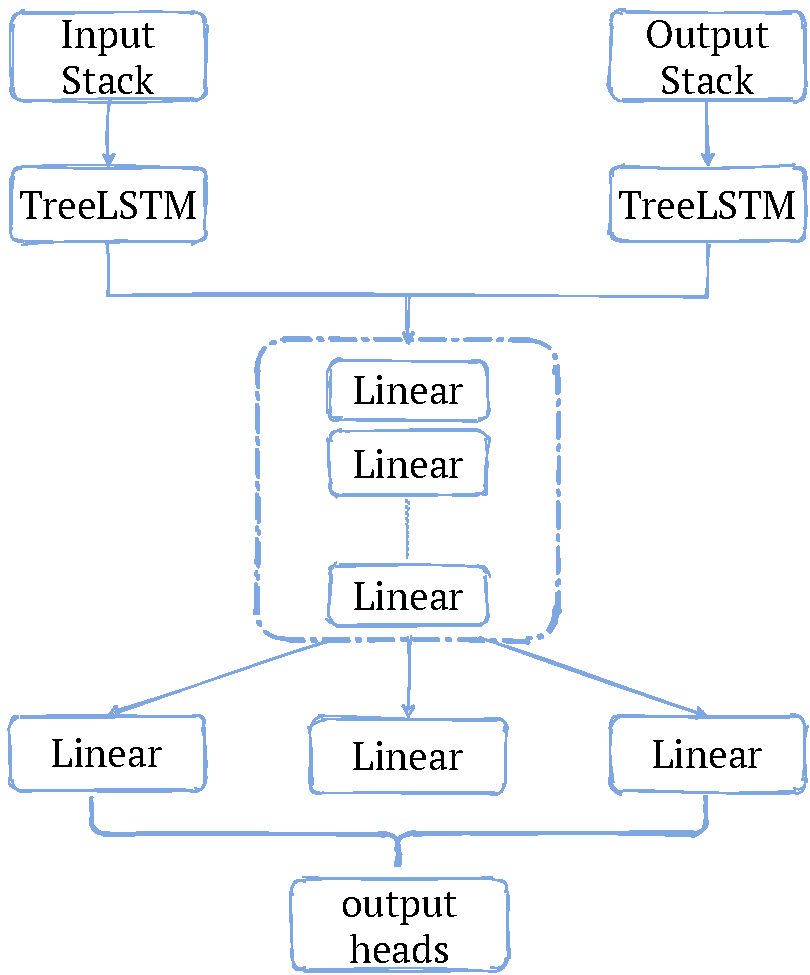
\includegraphics[width=0.4\textwidth]{nn.pdf}
    \caption{Network architecture}
    \label{fig:nn}
\end{figure}

In this stage, the \texttt{pytorch-tree-lstm} \cite{pytorch-tree-lstm} library helps the model increase efficiency in evaluating. Usually, efficient batching of tree data is complicated. It needs to evaluate all of a node's children before it can evaluate the node itself. To minimize the performance impact of this issue, the library breaks the node evaluation process into steps. In this way, each step it evaluates all nodes for which all child nodes have been previously evaluated. This allows the user to evaluate multiple nodes with each torch operation, increasing computation speeds by an order of magnitude over recursive approaches.

Take Figure \ref{fig:tree} for example, on the first step of the tree calculation, the library can evaluate nodes 1, Swap, 6, PNil and SNil in parallel as they are all leaves of the tree, i.e. none of them has any child nodes. At the second step, it will evaluate node Int, Instr, as their child nodes were evaluated previously. Finally, it evaluates node 0, which depends on nodes 1 and 2. By doing this, the library can reduce a 13-node computation to six steps. As the dataset gets larger and trees get bigger with more leaf nodes, the user can experience larger performance gains.

The network's output heads finally produce 3 vectors, corresponding to the three fields of \texttt{EncodeTerms} explained in Section \ref{sec:encoding} 

\begin{figure}[H]
    \centering
    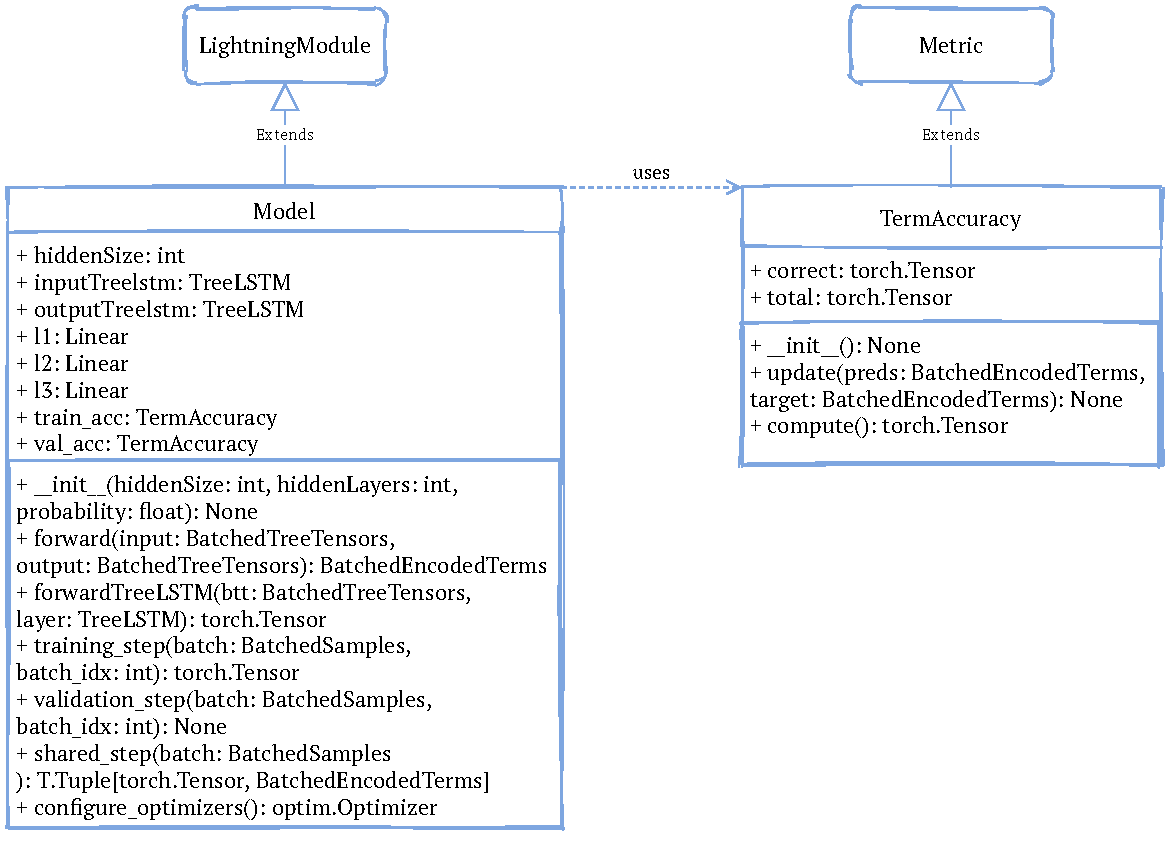
\includegraphics[width=1.02\textwidth]{classes.pdf}
    \caption{Model class and TermAccuracy class}
    \label{fig:classes}
\end{figure}

The image above is a class diagram for \texttt{Model} and \texttt{TermAccuracy}. They extends classes \texttt{LightningModule} and \texttt{Metric}, both of them are from the PyTorch Lightning \cite{pytorch-ligntning} library. Section \ref{sec:buildnn} to Section \ref{sec:train} goes through all the functions in the \texttt{Model} class, and Section \ref{sec:termacc} talks the class \texttt{TermAccuracy} in detail.

\subsection{Building the network}
\label{sec:buildnn}
Having seen the structure of the whole network, we are now going to see the implementation of it. 

Listing \ref{lst:cons} shows the constructor of the model. We have the number of nodes in each middle layer (\texttt{hiddenSize}), the number of hidden layers (\texttt{hiddenLayers}).

\begin{listing}[H]
\begin{minted}{python}
def __init__(self, hiddenSize: int, hiddenLayers: int):
    super().__init__()
    self.save_hyperparameters()
    self.hiddenSize = hiddenSize
    # Input layers
    self.inputTreelstm = TreeLSTM(len(labelClasses), hiddenSize)
    self.outputTreelstm = TreeLSTM(len(labelClasses), hiddenSize)
    # Hidden layers
    self.hidden = nn.ModuleList()
    for i in range(hiddenLayers):
        middle = nn.Linear(2 * hiddenSize, 2 * hiddenSize)
        self.hidden.append(middle)
    # Output layers
    self.l1 = nn.Linear(2 * hiddenSize, 1 + len(T.get_args(Value)))
    self.l2 = nn.Linear(2 * hiddenSize, 1 + len(T.get_args(Instruction)))
    self.l3 = nn.Linear(2 * hiddenSize, 1 + progIntRangeSize)
    
    self.train_acc = TermAccuracy()
    self.val_acc = TermAccuracy()
\end{minted}
\caption{Model constructor}
\label{lst:cons}
\end{listing}
We first create two Tree-LSTM layers for input and output stacks, the size of each input sample is the number of all the constructors for the abstract syntax tree and the number of features of the output of both layers is the hidden size. We concatenated two Tree-LSTM layers together before going through linear layers. Hence, the input and output size of middle layers are twofold of \texttt{hiddenSize}. Three output layers correspond to the output heads elaborated in \ref{sec:network}. 

\subsection{Applying layers}
Here follows how the input is processed through the network. We have \texttt{forwardTreeLSTM} and \texttt{forward} to do this job.

\texttt{forwardTreeLSTM} is used to apply Tree-LSTM layers to inputs. Four tensors \texttt{features}, \texttt{adjacency\_list}, \texttt{node\_order}, and \texttt{edge\_order} store the encoded tree structure and features.
Since the calculation of Tree-LSTM goes bottom up, we select the root nodes as the final result. The \texttt{unbatch\_tree\_tensor} is from the \texttt{pytorch-tree-lstm} library \cite{pytorch-tree-lstm}, it is used to unbatch the batched samples into a list. And we used \texttt{torch.unsqueeze} to create a new outer dimension to concatenate the samples.
\begin{listing}[H]
\begin{minted}{python}
def forwardTreeLSTM(self, btt: BatchedTreeTensors, layer: TreeLSTM) -> torch.Tensor:
    # Applying the layer.
    result, _ = layer(
        btt["features"].float(),
        btt["node_order"],
        btt["adjacency_list"],
        btt["edge_order"],
    )
    # Acquiring the calculated features of the root node for each sample.
    result = [
        torch.unsqueeze(sample[0], 0)
        for sample in unbatch_tree_tensor(result, btt["tree_sizes"])
    ]
    return torch.cat(result)
\end{minted}
\caption{Tree-LSTM layers}
\end{listing}

In \texttt{forward} ,the comment \mintinline{python}{type: ignore[override]} is used to silence the type checker on this line caused by incompatible overrides. Here we first concatenate two Tree-LSTM layers together, then use a for loop to add enough number of middle layers to the module list in the constructor and use \texttt{relu} activation function on each of them. And finally, return a tuple of three output heads. The class \texttt{BatchedEncodedTerms} has the same fields as \texttt{EncodedTerm} in Listing \ref{code:encodedTerm}, but the type of them is \texttt{torch.Tensor} instead of \texttt{int}.

\begin{listing}[H]
\begin{minted}{python}
def forward(  # type: ignore[override]
    self, input: BatchedTreeTensors, output: BatchedTreeTensors
) -> BatchedEncodedTerms:
    input1 = self.forwardTreeLSTM(input, self.inputTreelstm)
    input2 = self.forwardTreeLSTM(output, self.outputTreelstm)
    middle = torch.cat((input1, input2), 1)
    for i in range(len(self.hidden)):
        middle = self.hidden[i](middle)
        middle = nn.functional.layer_norm(middle, [self.hiddenSize * 2])
        middle = F.relu(middle)
    o1 = self.l1(middle)
    o2 = self.l2(middle)
    o3 = self.l3(middle)
    return BatchedEncodedTerms(o1, o2, o3)
\end{minted}
\caption{Network layers}
\end{listing}

\subsection{Training and improving model}
\label{sec:train}
\texttt{shared\_step} uses cross-entropy to measure the loss of three output tensors from the forward layer. It returns a tuple of the sum of the loss and the predicted result, and this step is necessary for both training and validation stages. \texttt{training\_step} and \texttt{validation\_step} are basically the same except that they used different datasets. 

\begin{listing}[H]
\begin{minted}{python}
def shared_step(
    self, batch: BatchedSamples
) -> T.Tuple[torch.Tensor, BatchedEncodedTerms]:
    predicted = self.forward(batch.input, batch.output)
    loss1 = nn.functional.cross_entropy(predicted.termLabel, batch.target.termLabel)
    loss2 = nn.functional.cross_entropy(
        predicted.instrLabel, batch.target.instrLabel
    )
    loss3 = nn.functional.cross_entropy(predicted.integer, batch.target.integer)
    return (loss1 + loss2 + loss3, predicted)
\end{minted}
\caption{The common step}
\end{listing}

\begin{listing}[H]
\begin{minted}{python}
def training_step(
    self, batch: BatchedSamples, batch_idx: int
) -> torch.Tensor:  # type: ignore[override]
    loss, predicted = self.shared_step(batch)
    accuracy = self.train_acc(predicted, batch.target)
    self.log("train_loss", loss)
    self.log("train_acc", accuracy, prog_bar=True)
    return loss

def validation_step(
    self, batch: BatchedSamples, batch_idx: int
) -> None:  # type: ignore[override]
    loss, predicted = self.shared_step(batch)
    accuracy = self.val_acc(predicted, batch.target)
    self.log("val_loss", loss, prog_bar=True)
    self.log("val_acc", accuracy, prog_bar=True)
\end{minted}
\caption{Training and validating}
\end{listing}

We used AdamW \cite{adamW} as the optimizer. It has an adaptive learning rate, with default parameter starting from 0.001. This enables it to solve problem of slower convergence in the late stage of training.
\begin{listing}[H]
\begin{minted}{python}
    def configure_optimizers(self) -> optim.Optimizer:
        return optim.AdamW(self.parameters())
\end{minted}
\caption{AdamW optimizer}
\end{listing}

\subsection{Measuring the accuracy}
\label{sec:termacc}
Evaluating the machine learning algorithm is an essential part of any project. Accuracy is one metric to measure how often the algorithm classifies a data point correctly. It is the ratio of the number of correct predictions to the total number of input samples.
\[Accuracy=\frac{Number\ of\ correct\ predictions}{Total\ number\ of\ predictions}\]

The accuracy of our model is measured by the sum of the three tensors generated by the output heads. We wrote our custom class for measuring it. \texttt{argmax} can find the class with the largest predicted probability.
\begin{listing}[H]
\begin{minted}{python}
class TermAccuracy(Metric):
    correct: torch.Tensor
    total: torch.Tensor
    def __init__(self) -> None:
        super().__init__()
        self.add_state("correct", default=torch.tensor(0), dist_reduce_fx="sum")
        self.add_state("total", default=torch.tensor(0), dist_reduce_fx="sum")

    def update(self, preds: BatchedEncodedTerms, target: BatchedEncodedTerms) -> None:
        t1 = torch.argmax(preds.termLabel, dim=1) == target.termLabel
        t2 = torch.argmax(preds.instrLabel, dim=1) == target.instrLabel
        t3 = torch.argmax(preds.integer, dim=1) == target.integer
        combined = torch.sum(t1 & t2 & t3)
        self.correct += combined
        self.total += torch.tensor(target.termLabel.numel())

    def compute(self) -> torch.Tensor:
        return self.correct.float() / self.total
\end{minted}
\caption{Custom Accuracy class}
\end{listing}


\subsection{Hyper-parameters and loss functions}
Hyper-parameters are parameters of the structure of the neural network, they can control the process of learning. We train our models with the following parameters:
\begin{itemize}
    \item Batch size: 32
    \item Middle layers: 5
    \item Hidden nodes: 1000
    \item Optimizer: AdamW
    \item Loss function: cross entropy
    \item Activation function: relu
\end{itemize}


\section{Testing}
\label{sec:test}
An application without testing is not trustworthy. Automated tests can be very useful for killing bugs in application development. It also keeps validating the code while adding new code or refactoring old code. 

There is a great number of functions that need to be tested in the project, and each function may need multiple test cases. Putting all the test cases into one \texttt{tests.py} file might not be a maintainable and scalable way. Therefore, we created a \texttt{tests} package in the root folder, and split tests into two folders \texttt{data} and \texttt{lang} to test files in the corresponding \texttt{data} and \texttt{lang} folder in the project. They also represent two main testings in this project. Pytest \cite{pytest} is for unit testing in \texttt{data} folder and hypothesis test \cite{hytest} is used for property testing in \texttt{lang} folder.


\subsection{Unit tests}
Python has built-in \texttt{unittest} module. It provides a solid base on which to build the test suite, but it has a few shortcomings. A number of third-party testing frameworks attempt to address some of the issues with \texttt{unittest}, and pytest \cite{pytestbook} has proven to be one of the most popular. It is a mature and full-featured testing framework, from small tests to large-scale functional tests for applications and libraries alike.

\dirtree{%
    .1 /data.
    .2 test\_deque.py.
    .2 test\_llist.py.
    .2 test\_stack.py.
    .2 test\_tree.py.
}

The structure above shows the files in \texttt{data} folder. With the powerful pytest library, we tested four main data structures: \texttt{deque}, \texttt{llist}, \texttt{stack}, and \texttt{tree}. For each data structure, we tested their main methods and the important functions related to them.

In \texttt{data/test\_deque.py}, we have the tests cases for the methods of double-ended queue data structure. Here are two examples, they test the \texttt{appendleft} method and the \texttt{pop} method of deque.
\begin{listing}[H]
\begin{minted}{python}
@given(st.lists(st.integers()), st.integers())
def test_deque_appendleft(xs: T.List[int], x: int) -> None:
    assert deque(xs).appendleft(x) == deque([x] + xs)

@given(st.lists(st.integers()).filter(lambda x: x))
def test_deque_pop(xs: T.List[int]) -> None:
    assert deque(xs).pop() == (deque(xs[:-1]), xs[-1])
\end{minted}
\caption{Part of Deque testing}
\end{listing}

\subsection{Property tests}
Property-based testing has become quite famous in the functional world. It relies on properties which means that it checks that a function, program, or whatever system under test abides by a property. Most of the time, properties do not have to go into too many details about the output. They just have to check for useful characteristics that must be seen in the output. 

Here is the content in the \texttt{lang} folder. For each function in \texttt{core.py}, \texttt{encodeStacks.py} and \texttt{encodeTerm.py} file, we gave one to three test cases.

\dirtree{%
    .1 /lang.
    .2 test\_core.py.
    .2 test\_encodeStacks.py.
    .2 test\_encodeTerm.py.
}

The following are some examples in the \texttt{test\_encodeStacks.py} file. For function \texttt{valueToTree}, we tested two types of the value - \texttt{Int} and \texttt{Quoted} separately. The same logic applies to \texttt{termToTree} as well, we tested two subtypes of the term, \texttt{Instr} and \texttt{Val}.
\begin{listing}[H]
\begin{minted}{python}
def test_valueToTree_Int() -> None:
    assert valueToTree(Int(3)) == Tree("Int", [Tree(3, [])])

def test_valueToTree_Quoted() -> None:
    assert valueToTree(Quoted(deque([Instr(Add())]))) == Tree(
        "Quoted", [Tree("PCons", [Tree("Instr", [Tree("Add", [])]), Tree("PNil", [])])]
    )
\end{minted}
\caption{Test valueToTree}
\end{listing}

\begin{listing}[H]
\begin{minted}{python}
def test_termToTree_Val() -> None:
    assert termToTree(Val(Int(8))) == Tree("Val", [Tree("Int", [Tree(8, [])])])

def test_termToTree_Instr() -> None:
    assert termToTree(Instr(Dup())) == Tree("Instr", [Tree("Dup", [])])
\end{minted}
\caption{Test termToTree}
\end{listing}

For the function \texttt{encodeStacks}, the one-hot encoded result is tested. The \texttt{stack1} and \texttt{stack2} are predefined. For the return value, we check whether each row contains only one 1 and everything else is 0.
\begin{listing}[H]
\begin{minted}{python}
def test_encodeStacks() -> None:
    features = encodeStacks((stack1, stack2))["features"]
    for row in features:
        num = numel(row)
        cnt = bincount(row.int())
        assert cnt[0] == num - 1
        assert cnt[1] == 1
\end{minted}
\caption{Test encodeStacks}
\end{listing}

For \texttt{progToTree}, \texttt{stackToTree} and \texttt{stacksToTree} in \texttt{encodeStacks.py} and \texttt{encodeInstr}, \texttt{encodeTerm} in \texttt{encodeTerm.py}, we calculate the desired result manually, and compare them with the function output. The following shows tests in \texttt{test\_encodeTerm.py} file.
\begin{listing}[H]
\begin{minted}{python}
def test_encodeInstr() -> None:
    assert encodeInstr(Swap()) == 1

def test_encodeTerm() -> None:
    assert encodeTerm(Val(Int(3))) == EncodedTerm(2, 0, 12)
\end{minted}
\caption{Test encodeTerm.py file}
\end{listing}

In \texttt{test\_core.py} file, three test cases are given for each of \texttt{quoteInstr}, \texttt{validateStack}, and \texttt{evalProgram} function. And to test \texttt{evalTerm} function, we wrote test cases for each instruction.

\subsection{Testing results}
There are by far 60 tests altogether. We tested all the major functions, but we can always add more test cases for the same function for the sake of safety. The command to run all the tests in the \texttt{tests} folder is: \texttt{python -m pytest}. You will see the following results.
{\small
\begin{verbatim}
================================= test session starts ==================================
platform darwin -- Python 3.8.6, pytest-6.2.2, py-1.10.0, pluggy-0.13.1
rootdir: /Users/su/Desktop/stack-prog-synth
plugins: hypothesis-6.2.0
collected 60 items                                                                         
tests/test_utils.py .                                                           [  1%]
tests/data/test_deque.py ...........                                            [ 20%]
tests/data/test_llist.py .                                                      [ 21%]
tests/data/test_stack.py .......                                                [ 33%]
tests/data/test_tree.py ..                                                      [ 36%]
tests/lang/test_core.py ......................                                  [ 73%]
tests/lang/test_encodeStacks.py ........                                        [ 86%]
tests/lang/test_encodeTerm.py ..                                                [ 90%]
tests/lang/test_type.py ......                                                  [100%]

================================== 60 passed in 5.96s ==================================
\end{verbatim}
}
\chapter{Conclusion}
The objective of this thesis was to design and implement software that can predict programs given user specifications and present to the user how the language works.

In the design phase, during the planning of the workflow, research was conducted on program synthesis, DSL, and Tree-LSTM networks. We chose Python as the programming language since Python code is understandable by humans, which makes it easier to build models for machine learning. And we decided to used PySimpleGUI to provide a graphical user interface. We found that it is more efficient and easier to work with if we construct our own domain-specific language.

In the implementation phase, we used many third-party tools to help us with the type checking and network building. We first implemented the DSL, then generated data with restrictions on integer ranges and validations on stack types, and encoded stacks. Then, we built the neural network, trained the model, and experimented with different hyper-parameters to improve the validation accuracy. 

The user interface is clean and stylish. It is able to guide the user step by step of how the composition of terms do their magic when manipulating the stack. By presenting the animation of the stack, the user can be more familiar with the stack data structure, and get the gist of the stack-oriented language.

Overall, the project achieved the desired result with an informative user interface. It is a helpful software for users who want to know more about program synthesis and stack-based programming paradigm.

\section*{Future Work}
\addcontentsline{toc}{section}{Future Work} 
The software is able to generate programs based on user specifications and provide a step-by-step demonstration to aid the user's understanding. But there are still many aspects that can be improved to be better. 

From the implementation perspective:
\begin{enumerate}
    \item In addition to \texttt{integers}, we can expand our language by including more types, such as \texttt{bool} and \texttt{list}.
    \item Implementing more instructions to make our DSL a Turing language.
    \item Improving our model with some hyperparameter optimization tools and introduce more complicated layers.
    \item For greater efficiency of the search algorithm, we can introduce the state-of-the-art best-first beam search \cite{best-first}.
\end{enumerate}

From the user perspective, we aim to develop more features to improve the user experience. For example, we plan to implement language translation. By converting our DSL to a lambda expression, then we can translate the lambda expression to other programming languages, such as python. This way, the user can export the language for later use.

% Lists
\clearpage
\phantomsection
\addcontentsline{toc}{chapter}{List of Figures}
\listoffigures

\clearpage
\phantomsection
\addcontentsline{toc}{chapter}{List of Listings}
\listoflistings

\clearpage
\phantomsection
\addcontentsline{toc}{chapter}{Bibliography}
\printbibliography

\end{document}